% lecture8.tex -- GENERATED by build_L8.py from L8_numbers.json; do not edit by hand.
\documentclass[10pt,aspectratio=169,t]{beamer}
% =============================================================================
% nn_preamble.tex -- shared Beamer preamble of Neural Networks and Deep Learning (NN)
% Used by every lecture: lectures/Lk/lecturek.tex does
%   \documentclass[10pt,aspectratio=169,t]{beamer}
%   % =============================================================================
% nn_preamble.tex -- shared Beamer preamble of Neural Networks and Deep Learning (NN)
% Used by every lecture: lectures/Lk/lecturek.tex does
%   \documentclass[10pt,aspectratio=169,t]{beamer}
%   % =============================================================================
% nn_preamble.tex -- shared Beamer preamble of Neural Networks and Deep Learning (NN)
% Used by every lecture: lectures/Lk/lecturek.tex does
%   \documentclass[10pt,aspectratio=169,t]{beamer}
%   \input{../common/nn_preamble}
%   \nnlecture{k}{Lecture title}
% Logos live in lectures/common/logos/, charts in lectures/Lk/charts/.
% Do NOT add \hfuzz / \vfuzz / \hbadness here: overfull boxes must be fixed, not hidden.
% =============================================================================

\usetheme{default}
\setbeamersize{text margin left=7mm, text margin right=7mm}

% ---------------------------------------------------------------- packages
\usepackage[utf8]{inputenc}
\usepackage[T1]{fontenc}
\usepackage{lmodern}
\usepackage{amsmath, amssymb}
\usepackage{mathtools}
\usepackage{bm}
\usepackage{tikz}
\usetikzlibrary{arrows.meta, positioning, calc, shapes.misc}
\usepackage{booktabs}
\usepackage{array}
\usepackage{graphicx}
\usepackage{colortbl}
\usepackage{xcolor}
\usepackage{multicol}
\hypersetup{colorlinks=true, linkcolor=MainBlue, urlcolor=MainBlue, citecolor=MainBlue}
\graphicspath{{../common/logos/}}   % charts are included with their language folder: charts/en/, charts/ro/

% ---------------------------------------------------------------- colours
\definecolor{MainBlue}{RGB}{26, 58, 110}
\definecolor{IDAred}{RGB}{205, 0, 0}
\definecolor{DarkGray}{RGB}{51, 51, 51}
\definecolor{FooterGray}{RGB}{100, 100, 100}
\definecolor{BlockGray}{RGB}{236, 238, 242}
\definecolor{KeynoteGray}{RGB}{218, 218, 218}
\definecolor{Crimson}{RGB}{190, 40, 50}
\definecolor{Forest}{RGB}{30, 110, 50}
\definecolor{Bitter}{RGB}{214, 150, 20}
% chart palette (same hex values and order as lectures/common/nn_plot.py SERIES)
\definecolor{Ser1}{HTML}{2A78D6}
\definecolor{Ser2}{HTML}{EB6834}
\definecolor{Ser3}{HTML}{1BAF7A}
\definecolor{Ser4}{HTML}{EDA100}
\definecolor{Ser5}{HTML}{E87BA4}
\definecolor{Ser6}{HTML}{008300}
\definecolor{Ser7}{HTML}{6250D6}
\definecolor{Ser8}{HTML}{E34948}

\setbeamertemplate{background}{%
  \begin{tikzpicture}[remember picture, overlay]
    \shade[shading=axis, shading angle=315, top color=white, bottom color=KeynoteGray]
      (current page.south west) rectangle (current page.north east);
  \end{tikzpicture}}
\setbeamercolor{background canvas}{bg=}
\setbeamercolor{structure}{fg=MainBlue}
\setbeamercolor{normal text}{fg=DarkGray}
\setbeamercolor{title}{fg=IDAred}
\setbeamercolor{frametitle}{fg=IDAred, bg=}
\setbeamercolor{block title}{bg=MainBlue, fg=white}
\setbeamercolor{block body}{bg=BlockGray, fg=DarkGray}
\setbeamercolor{block title alerted}{bg=Crimson, fg=white}
\setbeamercolor{block body alerted}{bg=Crimson!7, fg=DarkGray}
\setbeamercolor{block title example}{bg=Forest, fg=white}
\setbeamercolor{block body example}{bg=Forest!7, fg=DarkGray}
\setbeamercolor{item}{fg=MainBlue}
\setbeamerfont{frametitle}{size=\large, series=\bfseries}
\setbeamerfont{block title}{size=\small, series=\bfseries}
\setbeamertemplate{blocks}[rounded][shadow=false]
\setbeamertemplate{itemize item}{\color{MainBlue}$\boxdot$}
\setbeamertemplate{itemize subitem}{\color{MainBlue}\scriptsize$\blacktriangleright$}
% compact two-level lists: level 1 = main point, level 2 = details (no text outside bullets)
\setbeamerfont{itemize/enumerate subbody}{size=\footnotesize}
\setlength{\leftmargini}{1.1em}
\setlength{\leftmarginii}{1.1em}
\setbeamertemplate{itemize/enumerate body begin}{\setlength{\topsep}{0pt}\setlength{\partopsep}{0pt}\setlength{\parskip}{0pt}}
\setbeamertemplate{itemize/enumerate subbody begin}{\setlength{\topsep}{0pt}\setlength{\partopsep}{0pt}\setlength{\itemsep}{0pt}\vspace{-0.4ex}}

\setbeamertemplate{enumerate item}{\color{MainBlue}\insertenumlabel.}
\setlength{\leftmargini}{1.3em}
\setlength{\leftmarginii}{1.2em}
\setbeamertemplate{navigation symbols}{}
\setbeamertemplate{section in toc}{\color{MainBlue}$\blacktriangleright$~\inserttocsection}
\setbeamertemplate{caption}{\raggedright\insertcaption\par}
% frame subtitle = precise citation line under the claim title (Weron style)
\setbeamerfont{framesubtitle}{size=\footnotesize}
\setbeamercolor{framesubtitle}{fg=FooterGray}
% outline that reappears at every section with the current section highlighted
\setbeamertemplate{section in toc shaded}[default][35]
\setbeamertemplate{subsection in toc shaded}[default][35]
\setbeamertemplate{subsection in toc}{\leavevmode\leftskip=2.2em\color{DarkGray}\small\inserttocsubsection\par}
\AtBeginSection[]{{\begin{frame}{\txtoutline}\vspace{2mm}\small
  \tableofcontents[currentsection,hideothersubsections]\end{frame}}}

% ---------------------------------------------------------------- head and foot
\setbeamertemplate{headline}{%
  \vskip10pt%
  \hbox to \paperwidth{\hskip0.5cm%
    {\small\color{FooterGray}\renewcommand{\hyperlink}[2]{##2}\insertsectionhead}%
    \hfill\textcolor{FooterGray}{\small\insertframenumber}\hskip0.5cm}%
  \vskip4pt{\color{FooterGray}\hrule height 0.4pt}}
% footer as in the other courses (MFM, SFM): course name on the left, small sparkline on the right
\setbeamertemplate{footline}{%
  {\color{FooterGray}\hrule height 0.4pt}\vskip4pt%
  \hbox to \paperwidth{\hskip0.5cm%
    \textcolor{FooterGray}{\small\txtcourse}%
    \hfill\raisebox{-0.1em}{\begin{tikzpicture}[x=0.08em, y=0.08em, line width=0.4pt]
      \draw[FooterGray] (0,3) -- (1,4) -- (2,3.5) -- (3,5) -- (4,4) -- (5,6) -- (6,5.5) -- (7,4) -- (8,5) -- (9,7) -- (10,6) -- (11,5) -- (12,6.5) -- (13,8) -- (14,7) -- (15,6) -- (16,7.5) -- (17,9) -- (18,8) -- (19,7) -- (20,8.5) -- (21,10) -- (22,9) -- (23,8) -- (24,9.5);
    \end{tikzpicture}}\hskip0.5cm}%
  \vskip6pt}

% ---------------------------------------------------------------- title page
\defbeamertemplate*{title page}{nn}[1][]{%
  \vspace{0.15cm}
  \begin{center}
    \href{https://www.ase.ro}{
\includegraphics[height=0.9cm]{ase_logo.png}}\hspace{0.3cm}%
    \href{https://ipe.ro/new}{
\includegraphics[height=0.9cm]{acad_logo.png}}\hspace{0.3cm}%
    \href{https://theida.net}{
\includegraphics[height=0.9cm]{ida_logo.png}}\hspace{0.3cm}%
    \href{https://blockchain-research-center.com}{
\includegraphics[height=0.9cm]{brc_logo.png}}\hspace{0.3cm}%
    \href{https://www.ai4efin.ase.ro}{
\includegraphics[height=0.9cm]{ai4efin_logo.png}}\hspace{0.3cm}%
    \href{https://www.digital-finance-msca.com}{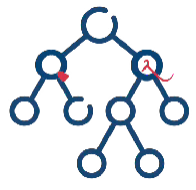
\includegraphics[height=0.9cm]{msca_logo.png}}%
  \end{center}
  \vspace{0.45cm}
  \begin{center}
    \begin{minipage}{0.1\textwidth}\centering
      \href{https://quantlet.com}{
\includegraphics[height=0.9cm]{ql_logo.png}}\end{minipage}%
    \begin{minipage}{0.78\textwidth}\centering
      {\Large\bfseries\usebeamercolor[fg]{title}\inserttitle}\par\vspace{0.25cm}
      {\large\usebeamercolor[fg]{title}\insertsubtitle}\end{minipage}%
    \begin{minipage}{0.1\textwidth}\centering
      \href{https://quantinar.com}{
\includegraphics[height=0.9cm]{qr_logo.png}}\end{minipage}
  \end{center}
  \vfill
  \hspace{0.4cm}{\bfseries\insertauthor}\par\vspace{0.12cm}
  \hspace{0.4cm}\begin{minipage}[t]{0.92\textwidth}\raggedright\footnotesize\insertinstitute\end{minipage}
  \par\vspace{0.4cm}}

% ---------------------------------------------------------------- lecture metadata
\newcommand{\nnshort}{}
\newcommand{\nnnb}{notebooks}
\newcommand{\nnrepo}{https://github.com/danpele/NEURAL_BIZ/tree/main}
% language-dependent labels (English default; \nnromanian switches to Romanian, call it before \nnlecture)
\newcommand{\txtcourse}{Neural Networks and Deep Learning}
\newcommand{\txtlecture}{Lecture}
\newcommand{\txtoutline}{Outline}
\newcommand{\txtintuition}{In one sentence:}
\newcommand{\txtjob}{In practice:}
\newcommand{\txttry}{Experiment yourself:}
\newcommand{\txtwhere}{where}
\newcommand{\txtsim}{SIMULATED DATA (teaching illustration)}
\newcommand{\txtnbsuffix}{}
\newcommand{\txtinstitute}{Bucharest University of Economic Studies (ASE), Department of Statistics and Econometrics\\
    Romanian Academy, Institute for Economic Forecasting (IPE)\\
    IDA Institute Digital Assets \textbullet\ AI4EFin \textbullet\ MSCA Digital Finance}
\newcommand{\nnromanian}{%
  \renewcommand{\txtcourse}{Rețele neuronale și deep learning}%
  \renewcommand{\txtlecture}{Cursul}%
  \renewcommand{\txtoutline}{Cuprins}%
  \renewcommand{\txtintuition}{Pe scurt:}%
  \renewcommand{\txtjob}{În practică:}%
  \renewcommand{\txttry}{Exercițiu practic:}%
  \renewcommand{\txtwhere}{unde}%
  \renewcommand{\txtsim}{DATE SIMULATE (doar pentru ilustrare)}%
  \renewcommand{\txtnbsuffix}{\string_ro}%
  \renewcommand{\txtinstitute}{Academia de Studii Economice din București (ASE), Departamentul de Statistică și Econometrie\\
    Academia Română, Institutul de Prognoză Economică (IPE)\\
    IDA Institute Digital Assets \textbullet\ AI4EFin \textbullet\ MSCA Digital Finance}}
\newcommand{\nnlecture}[2]{%
  \renewcommand{\nnshort}{\txtlecture\ #1}%
  \renewcommand{\nnnb}{notebooks/L#1\string_notebook\txtnbsuffix.ipynb}%
  \title[NN]{\txtcourse}%
  \subtitle{\txtlecture\ #1: #2}%
  \author{Prof.\ dr.\ Daniel Traian PELE}%
  \institute{\txtinstitute}%
  \date{}}

% ---------------------------------------------------------------- teaching blocks (one message per frame)
% \intuition{one plain sentence}  ->  formula with every symbol defined  ->  real-data example  ->  \manager{one line}
\newcommand{\intuition}[1]{\begin{itemize}\item {\color{MainBlue}\textbf{\txtintuition}}~#1\end{itemize}\vspace{0.6mm}}
\newcommand{\manager}[1]{\colorbox{Forest!10}{\parbox{\dimexpr\linewidth-2\fboxsep\relax}{\footnotesize
  \begin{itemize}\setlength{\itemsep}{0pt}\item \textbf{\color{Forest}\txtjob}~#1\end{itemize}}}}
% Experiment yourself: pointer to the matching notebook section
\newcommand{\tryit}[1]{{\scriptsize\href{\nnrepo/\nnnb}{%
  \raisebox{-0.15em}{
\includegraphics[height=0.85em]{ql_logo.png}}\,\textbf{\txttry}~\color{MainBlue}#1}}}
% bottom row: manager line (left) + experiment pointer (right), pinned to the bottom of the frame
\newcommand{\bottomrow}[2]{\par\vfill\noindent\begin{minipage}[b]{0.72\linewidth}#1\end{minipage}\hfill
  \begin{minipage}[b]{0.26\linewidth}\raggedleft #2\end{minipage}\par\vspace{0.5mm}}
\newcommand{\where}[1]{{\footnotesize\textbf{\txtwhere}~#1\par}}

% ---------------------------------------------------------------- helpers
% chart source line under a figure: \chartsource{Source ...; period ...}
\newcommand{\chartsource}[1]{\par\vspace{1pt}{\scriptsize\color{FooterGray}#1\par}}
% link to code: \quantlet{label}{path inside the repo}
\newcommand{\quantlet}[2]{\par\vspace{1pt}\hfill\href{\nnrepo/#2}{%
  \raisebox{-0.15em}{
\includegraphics[height=0.75em]{ql_logo.png}}\textcolor{MainBlue}{\scriptsize\ #1}}}
% inline Quantlet link for the bottom-right corner of a frame: \qlink{label}{path inside the repo}
\newcommand{\qlink}[2]{{\scriptsize\href{\nnrepo/#2}{\raisebox{-0.15em}{
\includegraphics[height=0.85em]{ql_logo.png}}\,\textcolor{MainBlue}{#1}}}}
\newcommand{\simlabel}{\colorbox{Crimson!12}{\scriptsize\bfseries\color{Crimson}\txtsim}}
\newcommand{\E}{\mathbb{E}}
\newcommand{\Var}{\operatorname{Var}}
\newcommand{\Cov}{\operatorname{Cov}}
\newcommand{\Corr}{\operatorname{Corr}}
\newcommand{\asinh}{\operatorname{asinh}}
\newcommand{\iid}{\overset{\text{i.i.d.}}{\sim}}
\newcommand{\EUR}{EUR}
% deep-learning notation (Bishop & Bishop, 2024): vectors bold lower case, matrices bold upper case
\newcommand{\R}{\mathbb{R}}
\newcommand{\vx}{\mathbf{x}}
\newcommand{\vy}{\mathbf{y}}
\newcommand{\vz}{\mathbf{z}}
\newcommand{\vh}{\mathbf{h}}
\newcommand{\vw}{\mathbf{w}}
\newcommand{\vb}{\mathbf{b}}
\newcommand{\mW}{\mathbf{W}}
\newcommand{\mX}{\mathbf{X}}
\newcommand{\btheta}{\boldsymbol{\theta}}
\newcommand{\loss}{\mathcal{L}}
\newcommand{\dataset}{\mathcal{D}}
\DeclareMathOperator*{\argmin}{arg\,min}
\DeclareMathOperator*{\argmax}{arg\,max}
\DeclareMathOperator{\softmax}{softmax}
\DeclareMathOperator{\ReLU}{ReLU}
\DeclareMathOperator{\sigm}{\sigma}

%   \nnlecture{k}{Lecture title}
% Logos live in lectures/common/logos/, charts in lectures/Lk/charts/.
% Do NOT add \hfuzz / \vfuzz / \hbadness here: overfull boxes must be fixed, not hidden.
% =============================================================================

\usetheme{default}
\setbeamersize{text margin left=7mm, text margin right=7mm}

% ---------------------------------------------------------------- packages
\usepackage[utf8]{inputenc}
\usepackage[T1]{fontenc}
\usepackage{lmodern}
\usepackage{amsmath, amssymb}
\usepackage{mathtools}
\usepackage{bm}
\usepackage{tikz}
\usetikzlibrary{arrows.meta, positioning, calc, shapes.misc}
\usepackage{booktabs}
\usepackage{array}
\usepackage{graphicx}
\usepackage{colortbl}
\usepackage{xcolor}
\usepackage{multicol}
\hypersetup{colorlinks=true, linkcolor=MainBlue, urlcolor=MainBlue, citecolor=MainBlue}
\graphicspath{{../common/logos/}}   % charts are included with their language folder: charts/en/, charts/ro/

% ---------------------------------------------------------------- colours
\definecolor{MainBlue}{RGB}{26, 58, 110}
\definecolor{IDAred}{RGB}{205, 0, 0}
\definecolor{DarkGray}{RGB}{51, 51, 51}
\definecolor{FooterGray}{RGB}{100, 100, 100}
\definecolor{BlockGray}{RGB}{236, 238, 242}
\definecolor{KeynoteGray}{RGB}{218, 218, 218}
\definecolor{Crimson}{RGB}{190, 40, 50}
\definecolor{Forest}{RGB}{30, 110, 50}
\definecolor{Bitter}{RGB}{214, 150, 20}
% chart palette (same hex values and order as lectures/common/nn_plot.py SERIES)
\definecolor{Ser1}{HTML}{2A78D6}
\definecolor{Ser2}{HTML}{EB6834}
\definecolor{Ser3}{HTML}{1BAF7A}
\definecolor{Ser4}{HTML}{EDA100}
\definecolor{Ser5}{HTML}{E87BA4}
\definecolor{Ser6}{HTML}{008300}
\definecolor{Ser7}{HTML}{6250D6}
\definecolor{Ser8}{HTML}{E34948}

\setbeamertemplate{background}{%
  \begin{tikzpicture}[remember picture, overlay]
    \shade[shading=axis, shading angle=315, top color=white, bottom color=KeynoteGray]
      (current page.south west) rectangle (current page.north east);
  \end{tikzpicture}}
\setbeamercolor{background canvas}{bg=}
\setbeamercolor{structure}{fg=MainBlue}
\setbeamercolor{normal text}{fg=DarkGray}
\setbeamercolor{title}{fg=IDAred}
\setbeamercolor{frametitle}{fg=IDAred, bg=}
\setbeamercolor{block title}{bg=MainBlue, fg=white}
\setbeamercolor{block body}{bg=BlockGray, fg=DarkGray}
\setbeamercolor{block title alerted}{bg=Crimson, fg=white}
\setbeamercolor{block body alerted}{bg=Crimson!7, fg=DarkGray}
\setbeamercolor{block title example}{bg=Forest, fg=white}
\setbeamercolor{block body example}{bg=Forest!7, fg=DarkGray}
\setbeamercolor{item}{fg=MainBlue}
\setbeamerfont{frametitle}{size=\large, series=\bfseries}
\setbeamerfont{block title}{size=\small, series=\bfseries}
\setbeamertemplate{blocks}[rounded][shadow=false]
\setbeamertemplate{itemize item}{\color{MainBlue}$\boxdot$}
\setbeamertemplate{itemize subitem}{\color{MainBlue}\scriptsize$\blacktriangleright$}
% compact two-level lists: level 1 = main point, level 2 = details (no text outside bullets)
\setbeamerfont{itemize/enumerate subbody}{size=\footnotesize}
\setlength{\leftmargini}{1.1em}
\setlength{\leftmarginii}{1.1em}
\setbeamertemplate{itemize/enumerate body begin}{\setlength{\topsep}{0pt}\setlength{\partopsep}{0pt}\setlength{\parskip}{0pt}}
\setbeamertemplate{itemize/enumerate subbody begin}{\setlength{\topsep}{0pt}\setlength{\partopsep}{0pt}\setlength{\itemsep}{0pt}\vspace{-0.4ex}}

\setbeamertemplate{enumerate item}{\color{MainBlue}\insertenumlabel.}
\setlength{\leftmargini}{1.3em}
\setlength{\leftmarginii}{1.2em}
\setbeamertemplate{navigation symbols}{}
\setbeamertemplate{section in toc}{\color{MainBlue}$\blacktriangleright$~\inserttocsection}
\setbeamertemplate{caption}{\raggedright\insertcaption\par}
% frame subtitle = precise citation line under the claim title (Weron style)
\setbeamerfont{framesubtitle}{size=\footnotesize}
\setbeamercolor{framesubtitle}{fg=FooterGray}
% outline that reappears at every section with the current section highlighted
\setbeamertemplate{section in toc shaded}[default][35]
\setbeamertemplate{subsection in toc shaded}[default][35]
\setbeamertemplate{subsection in toc}{\leavevmode\leftskip=2.2em\color{DarkGray}\small\inserttocsubsection\par}
\AtBeginSection[]{{\begin{frame}{\txtoutline}\vspace{2mm}\small
  \tableofcontents[currentsection,hideothersubsections]\end{frame}}}

% ---------------------------------------------------------------- head and foot
\setbeamertemplate{headline}{%
  \vskip10pt%
  \hbox to \paperwidth{\hskip0.5cm%
    {\small\color{FooterGray}\renewcommand{\hyperlink}[2]{##2}\insertsectionhead}%
    \hfill\textcolor{FooterGray}{\small\insertframenumber}\hskip0.5cm}%
  \vskip4pt{\color{FooterGray}\hrule height 0.4pt}}
% footer as in the other courses (MFM, SFM): course name on the left, small sparkline on the right
\setbeamertemplate{footline}{%
  {\color{FooterGray}\hrule height 0.4pt}\vskip4pt%
  \hbox to \paperwidth{\hskip0.5cm%
    \textcolor{FooterGray}{\small\txtcourse}%
    \hfill\raisebox{-0.1em}{\begin{tikzpicture}[x=0.08em, y=0.08em, line width=0.4pt]
      \draw[FooterGray] (0,3) -- (1,4) -- (2,3.5) -- (3,5) -- (4,4) -- (5,6) -- (6,5.5) -- (7,4) -- (8,5) -- (9,7) -- (10,6) -- (11,5) -- (12,6.5) -- (13,8) -- (14,7) -- (15,6) -- (16,7.5) -- (17,9) -- (18,8) -- (19,7) -- (20,8.5) -- (21,10) -- (22,9) -- (23,8) -- (24,9.5);
    \end{tikzpicture}}\hskip0.5cm}%
  \vskip6pt}

% ---------------------------------------------------------------- title page
\defbeamertemplate*{title page}{nn}[1][]{%
  \vspace{0.15cm}
  \begin{center}
    \href{https://www.ase.ro}{
\includegraphics[height=0.9cm]{ase_logo.png}}\hspace{0.3cm}%
    \href{https://ipe.ro/new}{
\includegraphics[height=0.9cm]{acad_logo.png}}\hspace{0.3cm}%
    \href{https://theida.net}{
\includegraphics[height=0.9cm]{ida_logo.png}}\hspace{0.3cm}%
    \href{https://blockchain-research-center.com}{
\includegraphics[height=0.9cm]{brc_logo.png}}\hspace{0.3cm}%
    \href{https://www.ai4efin.ase.ro}{
\includegraphics[height=0.9cm]{ai4efin_logo.png}}\hspace{0.3cm}%
    \href{https://www.digital-finance-msca.com}{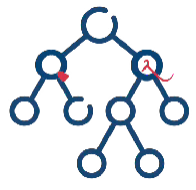
\includegraphics[height=0.9cm]{msca_logo.png}}%
  \end{center}
  \vspace{0.45cm}
  \begin{center}
    \begin{minipage}{0.1\textwidth}\centering
      \href{https://quantlet.com}{
\includegraphics[height=0.9cm]{ql_logo.png}}\end{minipage}%
    \begin{minipage}{0.78\textwidth}\centering
      {\Large\bfseries\usebeamercolor[fg]{title}\inserttitle}\par\vspace{0.25cm}
      {\large\usebeamercolor[fg]{title}\insertsubtitle}\end{minipage}%
    \begin{minipage}{0.1\textwidth}\centering
      \href{https://quantinar.com}{
\includegraphics[height=0.9cm]{qr_logo.png}}\end{minipage}
  \end{center}
  \vfill
  \hspace{0.4cm}{\bfseries\insertauthor}\par\vspace{0.12cm}
  \hspace{0.4cm}\begin{minipage}[t]{0.92\textwidth}\raggedright\footnotesize\insertinstitute\end{minipage}
  \par\vspace{0.4cm}}

% ---------------------------------------------------------------- lecture metadata
\newcommand{\nnshort}{}
\newcommand{\nnnb}{notebooks}
\newcommand{\nnrepo}{https://github.com/danpele/NEURAL_BIZ/tree/main}
% language-dependent labels (English default; \nnromanian switches to Romanian, call it before \nnlecture)
\newcommand{\txtcourse}{Neural Networks and Deep Learning}
\newcommand{\txtlecture}{Lecture}
\newcommand{\txtoutline}{Outline}
\newcommand{\txtintuition}{In one sentence:}
\newcommand{\txtjob}{In practice:}
\newcommand{\txttry}{Experiment yourself:}
\newcommand{\txtwhere}{where}
\newcommand{\txtsim}{SIMULATED DATA (teaching illustration)}
\newcommand{\txtnbsuffix}{}
\newcommand{\txtinstitute}{Bucharest University of Economic Studies (ASE), Department of Statistics and Econometrics\\
    Romanian Academy, Institute for Economic Forecasting (IPE)\\
    IDA Institute Digital Assets \textbullet\ AI4EFin \textbullet\ MSCA Digital Finance}
\newcommand{\nnromanian}{%
  \renewcommand{\txtcourse}{Rețele neuronale și deep learning}%
  \renewcommand{\txtlecture}{Cursul}%
  \renewcommand{\txtoutline}{Cuprins}%
  \renewcommand{\txtintuition}{Pe scurt:}%
  \renewcommand{\txtjob}{În practică:}%
  \renewcommand{\txttry}{Exercițiu practic:}%
  \renewcommand{\txtwhere}{unde}%
  \renewcommand{\txtsim}{DATE SIMULATE (doar pentru ilustrare)}%
  \renewcommand{\txtnbsuffix}{\string_ro}%
  \renewcommand{\txtinstitute}{Academia de Studii Economice din București (ASE), Departamentul de Statistică și Econometrie\\
    Academia Română, Institutul de Prognoză Economică (IPE)\\
    IDA Institute Digital Assets \textbullet\ AI4EFin \textbullet\ MSCA Digital Finance}}
\newcommand{\nnlecture}[2]{%
  \renewcommand{\nnshort}{\txtlecture\ #1}%
  \renewcommand{\nnnb}{notebooks/L#1\string_notebook\txtnbsuffix.ipynb}%
  \title[NN]{\txtcourse}%
  \subtitle{\txtlecture\ #1: #2}%
  \author{Prof.\ dr.\ Daniel Traian PELE}%
  \institute{\txtinstitute}%
  \date{}}

% ---------------------------------------------------------------- teaching blocks (one message per frame)
% \intuition{one plain sentence}  ->  formula with every symbol defined  ->  real-data example  ->  \manager{one line}
\newcommand{\intuition}[1]{\begin{itemize}\item {\color{MainBlue}\textbf{\txtintuition}}~#1\end{itemize}\vspace{0.6mm}}
\newcommand{\manager}[1]{\colorbox{Forest!10}{\parbox{\dimexpr\linewidth-2\fboxsep\relax}{\footnotesize
  \begin{itemize}\setlength{\itemsep}{0pt}\item \textbf{\color{Forest}\txtjob}~#1\end{itemize}}}}
% Experiment yourself: pointer to the matching notebook section
\newcommand{\tryit}[1]{{\scriptsize\href{\nnrepo/\nnnb}{%
  \raisebox{-0.15em}{
\includegraphics[height=0.85em]{ql_logo.png}}\,\textbf{\txttry}~\color{MainBlue}#1}}}
% bottom row: manager line (left) + experiment pointer (right), pinned to the bottom of the frame
\newcommand{\bottomrow}[2]{\par\vfill\noindent\begin{minipage}[b]{0.72\linewidth}#1\end{minipage}\hfill
  \begin{minipage}[b]{0.26\linewidth}\raggedleft #2\end{minipage}\par\vspace{0.5mm}}
\newcommand{\where}[1]{{\footnotesize\textbf{\txtwhere}~#1\par}}

% ---------------------------------------------------------------- helpers
% chart source line under a figure: \chartsource{Source ...; period ...}
\newcommand{\chartsource}[1]{\par\vspace{1pt}{\scriptsize\color{FooterGray}#1\par}}
% link to code: \quantlet{label}{path inside the repo}
\newcommand{\quantlet}[2]{\par\vspace{1pt}\hfill\href{\nnrepo/#2}{%
  \raisebox{-0.15em}{
\includegraphics[height=0.75em]{ql_logo.png}}\textcolor{MainBlue}{\scriptsize\ #1}}}
% inline Quantlet link for the bottom-right corner of a frame: \qlink{label}{path inside the repo}
\newcommand{\qlink}[2]{{\scriptsize\href{\nnrepo/#2}{\raisebox{-0.15em}{
\includegraphics[height=0.85em]{ql_logo.png}}\,\textcolor{MainBlue}{#1}}}}
\newcommand{\simlabel}{\colorbox{Crimson!12}{\scriptsize\bfseries\color{Crimson}\txtsim}}
\newcommand{\E}{\mathbb{E}}
\newcommand{\Var}{\operatorname{Var}}
\newcommand{\Cov}{\operatorname{Cov}}
\newcommand{\Corr}{\operatorname{Corr}}
\newcommand{\asinh}{\operatorname{asinh}}
\newcommand{\iid}{\overset{\text{i.i.d.}}{\sim}}
\newcommand{\EUR}{EUR}
% deep-learning notation (Bishop & Bishop, 2024): vectors bold lower case, matrices bold upper case
\newcommand{\R}{\mathbb{R}}
\newcommand{\vx}{\mathbf{x}}
\newcommand{\vy}{\mathbf{y}}
\newcommand{\vz}{\mathbf{z}}
\newcommand{\vh}{\mathbf{h}}
\newcommand{\vw}{\mathbf{w}}
\newcommand{\vb}{\mathbf{b}}
\newcommand{\mW}{\mathbf{W}}
\newcommand{\mX}{\mathbf{X}}
\newcommand{\btheta}{\boldsymbol{\theta}}
\newcommand{\loss}{\mathcal{L}}
\newcommand{\dataset}{\mathcal{D}}
\DeclareMathOperator*{\argmin}{arg\,min}
\DeclareMathOperator*{\argmax}{arg\,max}
\DeclareMathOperator{\softmax}{softmax}
\DeclareMathOperator{\ReLU}{ReLU}
\DeclareMathOperator{\sigm}{\sigma}

%   \nnlecture{k}{Lecture title}
% Logos live in lectures/common/logos/, charts in lectures/Lk/charts/.
% Do NOT add \hfuzz / \vfuzz / \hbadness here: overfull boxes must be fixed, not hidden.
% =============================================================================

\usetheme{default}
\setbeamersize{text margin left=7mm, text margin right=7mm}

% ---------------------------------------------------------------- packages
\usepackage[utf8]{inputenc}
\usepackage[T1]{fontenc}
\usepackage{lmodern}
\usepackage{amsmath, amssymb}
\usepackage{mathtools}
\usepackage{bm}
\usepackage{tikz}
\usetikzlibrary{arrows.meta, positioning, calc, shapes.misc}
\usepackage{booktabs}
\usepackage{array}
\usepackage{graphicx}
\usepackage{colortbl}
\usepackage{xcolor}
\usepackage{multicol}
\hypersetup{colorlinks=true, linkcolor=MainBlue, urlcolor=MainBlue, citecolor=MainBlue}
\graphicspath{{../common/logos/}}   % charts are included with their language folder: charts/en/, charts/ro/

% ---------------------------------------------------------------- colours
\definecolor{MainBlue}{RGB}{26, 58, 110}
\definecolor{IDAred}{RGB}{205, 0, 0}
\definecolor{DarkGray}{RGB}{51, 51, 51}
\definecolor{FooterGray}{RGB}{100, 100, 100}
\definecolor{BlockGray}{RGB}{236, 238, 242}
\definecolor{KeynoteGray}{RGB}{218, 218, 218}
\definecolor{Crimson}{RGB}{190, 40, 50}
\definecolor{Forest}{RGB}{30, 110, 50}
\definecolor{Bitter}{RGB}{214, 150, 20}
% chart palette (same hex values and order as lectures/common/nn_plot.py SERIES)
\definecolor{Ser1}{HTML}{2A78D6}
\definecolor{Ser2}{HTML}{EB6834}
\definecolor{Ser3}{HTML}{1BAF7A}
\definecolor{Ser4}{HTML}{EDA100}
\definecolor{Ser5}{HTML}{E87BA4}
\definecolor{Ser6}{HTML}{008300}
\definecolor{Ser7}{HTML}{6250D6}
\definecolor{Ser8}{HTML}{E34948}

\setbeamertemplate{background}{%
  \begin{tikzpicture}[remember picture, overlay]
    \shade[shading=axis, shading angle=315, top color=white, bottom color=KeynoteGray]
      (current page.south west) rectangle (current page.north east);
  \end{tikzpicture}}
\setbeamercolor{background canvas}{bg=}
\setbeamercolor{structure}{fg=MainBlue}
\setbeamercolor{normal text}{fg=DarkGray}
\setbeamercolor{title}{fg=IDAred}
\setbeamercolor{frametitle}{fg=IDAred, bg=}
\setbeamercolor{block title}{bg=MainBlue, fg=white}
\setbeamercolor{block body}{bg=BlockGray, fg=DarkGray}
\setbeamercolor{block title alerted}{bg=Crimson, fg=white}
\setbeamercolor{block body alerted}{bg=Crimson!7, fg=DarkGray}
\setbeamercolor{block title example}{bg=Forest, fg=white}
\setbeamercolor{block body example}{bg=Forest!7, fg=DarkGray}
\setbeamercolor{item}{fg=MainBlue}
\setbeamerfont{frametitle}{size=\large, series=\bfseries}
\setbeamerfont{block title}{size=\small, series=\bfseries}
\setbeamertemplate{blocks}[rounded][shadow=false]
\setbeamertemplate{itemize item}{\color{MainBlue}$\boxdot$}
\setbeamertemplate{itemize subitem}{\color{MainBlue}\scriptsize$\blacktriangleright$}
% compact two-level lists: level 1 = main point, level 2 = details (no text outside bullets)
\setbeamerfont{itemize/enumerate subbody}{size=\footnotesize}
\setlength{\leftmargini}{1.1em}
\setlength{\leftmarginii}{1.1em}
\setbeamertemplate{itemize/enumerate body begin}{\setlength{\topsep}{0pt}\setlength{\partopsep}{0pt}\setlength{\parskip}{0pt}}
\setbeamertemplate{itemize/enumerate subbody begin}{\setlength{\topsep}{0pt}\setlength{\partopsep}{0pt}\setlength{\itemsep}{0pt}\vspace{-0.4ex}}

\setbeamertemplate{enumerate item}{\color{MainBlue}\insertenumlabel.}
\setlength{\leftmargini}{1.3em}
\setlength{\leftmarginii}{1.2em}
\setbeamertemplate{navigation symbols}{}
\setbeamertemplate{section in toc}{\color{MainBlue}$\blacktriangleright$~\inserttocsection}
\setbeamertemplate{caption}{\raggedright\insertcaption\par}
% frame subtitle = precise citation line under the claim title (Weron style)
\setbeamerfont{framesubtitle}{size=\footnotesize}
\setbeamercolor{framesubtitle}{fg=FooterGray}
% outline that reappears at every section with the current section highlighted
\setbeamertemplate{section in toc shaded}[default][35]
\setbeamertemplate{subsection in toc shaded}[default][35]
\setbeamertemplate{subsection in toc}{\leavevmode\leftskip=2.2em\color{DarkGray}\small\inserttocsubsection\par}
\AtBeginSection[]{{\begin{frame}{\txtoutline}\vspace{2mm}\small
  \tableofcontents[currentsection,hideothersubsections]\end{frame}}}

% ---------------------------------------------------------------- head and foot
\setbeamertemplate{headline}{%
  \vskip10pt%
  \hbox to \paperwidth{\hskip0.5cm%
    {\small\color{FooterGray}\renewcommand{\hyperlink}[2]{##2}\insertsectionhead}%
    \hfill\textcolor{FooterGray}{\small\insertframenumber}\hskip0.5cm}%
  \vskip4pt{\color{FooterGray}\hrule height 0.4pt}}
% footer as in the other courses (MFM, SFM): course name on the left, small sparkline on the right
\setbeamertemplate{footline}{%
  {\color{FooterGray}\hrule height 0.4pt}\vskip4pt%
  \hbox to \paperwidth{\hskip0.5cm%
    \textcolor{FooterGray}{\small\txtcourse}%
    \hfill\raisebox{-0.1em}{\begin{tikzpicture}[x=0.08em, y=0.08em, line width=0.4pt]
      \draw[FooterGray] (0,3) -- (1,4) -- (2,3.5) -- (3,5) -- (4,4) -- (5,6) -- (6,5.5) -- (7,4) -- (8,5) -- (9,7) -- (10,6) -- (11,5) -- (12,6.5) -- (13,8) -- (14,7) -- (15,6) -- (16,7.5) -- (17,9) -- (18,8) -- (19,7) -- (20,8.5) -- (21,10) -- (22,9) -- (23,8) -- (24,9.5);
    \end{tikzpicture}}\hskip0.5cm}%
  \vskip6pt}

% ---------------------------------------------------------------- title page
\defbeamertemplate*{title page}{nn}[1][]{%
  \vspace{0.15cm}
  \begin{center}
    \href{https://www.ase.ro}{
\includegraphics[height=0.9cm]{ase_logo.png}}\hspace{0.3cm}%
    \href{https://ipe.ro/new}{
\includegraphics[height=0.9cm]{acad_logo.png}}\hspace{0.3cm}%
    \href{https://theida.net}{
\includegraphics[height=0.9cm]{ida_logo.png}}\hspace{0.3cm}%
    \href{https://blockchain-research-center.com}{
\includegraphics[height=0.9cm]{brc_logo.png}}\hspace{0.3cm}%
    \href{https://www.ai4efin.ase.ro}{
\includegraphics[height=0.9cm]{ai4efin_logo.png}}\hspace{0.3cm}%
    \href{https://www.digital-finance-msca.com}{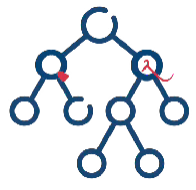
\includegraphics[height=0.9cm]{msca_logo.png}}%
  \end{center}
  \vspace{0.45cm}
  \begin{center}
    \begin{minipage}{0.1\textwidth}\centering
      \href{https://quantlet.com}{
\includegraphics[height=0.9cm]{ql_logo.png}}\end{minipage}%
    \begin{minipage}{0.78\textwidth}\centering
      {\Large\bfseries\usebeamercolor[fg]{title}\inserttitle}\par\vspace{0.25cm}
      {\large\usebeamercolor[fg]{title}\insertsubtitle}\end{minipage}%
    \begin{minipage}{0.1\textwidth}\centering
      \href{https://quantinar.com}{
\includegraphics[height=0.9cm]{qr_logo.png}}\end{minipage}
  \end{center}
  \vfill
  \hspace{0.4cm}{\bfseries\insertauthor}\par\vspace{0.12cm}
  \hspace{0.4cm}\begin{minipage}[t]{0.92\textwidth}\raggedright\footnotesize\insertinstitute\end{minipage}
  \par\vspace{0.4cm}}

% ---------------------------------------------------------------- lecture metadata
\newcommand{\nnshort}{}
\newcommand{\nnnb}{notebooks}
\newcommand{\nnrepo}{https://github.com/danpele/NEURAL_BIZ/tree/main}
% language-dependent labels (English default; \nnromanian switches to Romanian, call it before \nnlecture)
\newcommand{\txtcourse}{Neural Networks and Deep Learning}
\newcommand{\txtlecture}{Lecture}
\newcommand{\txtoutline}{Outline}
\newcommand{\txtintuition}{In one sentence:}
\newcommand{\txtjob}{In practice:}
\newcommand{\txttry}{Experiment yourself:}
\newcommand{\txtwhere}{where}
\newcommand{\txtsim}{SIMULATED DATA (teaching illustration)}
\newcommand{\txtnbsuffix}{}
\newcommand{\txtinstitute}{Bucharest University of Economic Studies (ASE), Department of Statistics and Econometrics\\
    Romanian Academy, Institute for Economic Forecasting (IPE)\\
    IDA Institute Digital Assets \textbullet\ AI4EFin \textbullet\ MSCA Digital Finance}
\newcommand{\nnromanian}{%
  \renewcommand{\txtcourse}{Rețele neuronale și deep learning}%
  \renewcommand{\txtlecture}{Cursul}%
  \renewcommand{\txtoutline}{Cuprins}%
  \renewcommand{\txtintuition}{Pe scurt:}%
  \renewcommand{\txtjob}{În practică:}%
  \renewcommand{\txttry}{Exercițiu practic:}%
  \renewcommand{\txtwhere}{unde}%
  \renewcommand{\txtsim}{DATE SIMULATE (doar pentru ilustrare)}%
  \renewcommand{\txtnbsuffix}{\string_ro}%
  \renewcommand{\txtinstitute}{Academia de Studii Economice din București (ASE), Departamentul de Statistică și Econometrie\\
    Academia Română, Institutul de Prognoză Economică (IPE)\\
    IDA Institute Digital Assets \textbullet\ AI4EFin \textbullet\ MSCA Digital Finance}}
\newcommand{\nnlecture}[2]{%
  \renewcommand{\nnshort}{\txtlecture\ #1}%
  \renewcommand{\nnnb}{notebooks/L#1\string_notebook\txtnbsuffix.ipynb}%
  \title[NN]{\txtcourse}%
  \subtitle{\txtlecture\ #1: #2}%
  \author{Prof.\ dr.\ Daniel Traian PELE}%
  \institute{\txtinstitute}%
  \date{}}

% ---------------------------------------------------------------- teaching blocks (one message per frame)
% \intuition{one plain sentence}  ->  formula with every symbol defined  ->  real-data example  ->  \manager{one line}
\newcommand{\intuition}[1]{\begin{itemize}\item {\color{MainBlue}\textbf{\txtintuition}}~#1\end{itemize}\vspace{0.6mm}}
\newcommand{\manager}[1]{\colorbox{Forest!10}{\parbox{\dimexpr\linewidth-2\fboxsep\relax}{\footnotesize
  \begin{itemize}\setlength{\itemsep}{0pt}\item \textbf{\color{Forest}\txtjob}~#1\end{itemize}}}}
% Experiment yourself: pointer to the matching notebook section
\newcommand{\tryit}[1]{{\scriptsize\href{\nnrepo/\nnnb}{%
  \raisebox{-0.15em}{
\includegraphics[height=0.85em]{ql_logo.png}}\,\textbf{\txttry}~\color{MainBlue}#1}}}
% bottom row: manager line (left) + experiment pointer (right), pinned to the bottom of the frame
\newcommand{\bottomrow}[2]{\par\vfill\noindent\begin{minipage}[b]{0.72\linewidth}#1\end{minipage}\hfill
  \begin{minipage}[b]{0.26\linewidth}\raggedleft #2\end{minipage}\par\vspace{0.5mm}}
\newcommand{\where}[1]{{\footnotesize\textbf{\txtwhere}~#1\par}}

% ---------------------------------------------------------------- helpers
% chart source line under a figure: \chartsource{Source ...; period ...}
\newcommand{\chartsource}[1]{\par\vspace{1pt}{\scriptsize\color{FooterGray}#1\par}}
% link to code: \quantlet{label}{path inside the repo}
\newcommand{\quantlet}[2]{\par\vspace{1pt}\hfill\href{\nnrepo/#2}{%
  \raisebox{-0.15em}{
\includegraphics[height=0.75em]{ql_logo.png}}\textcolor{MainBlue}{\scriptsize\ #1}}}
% inline Quantlet link for the bottom-right corner of a frame: \qlink{label}{path inside the repo}
\newcommand{\qlink}[2]{{\scriptsize\href{\nnrepo/#2}{\raisebox{-0.15em}{
\includegraphics[height=0.85em]{ql_logo.png}}\,\textcolor{MainBlue}{#1}}}}
\newcommand{\simlabel}{\colorbox{Crimson!12}{\scriptsize\bfseries\color{Crimson}\txtsim}}
\newcommand{\E}{\mathbb{E}}
\newcommand{\Var}{\operatorname{Var}}
\newcommand{\Cov}{\operatorname{Cov}}
\newcommand{\Corr}{\operatorname{Corr}}
\newcommand{\asinh}{\operatorname{asinh}}
\newcommand{\iid}{\overset{\text{i.i.d.}}{\sim}}
\newcommand{\EUR}{EUR}
% deep-learning notation (Bishop & Bishop, 2024): vectors bold lower case, matrices bold upper case
\newcommand{\R}{\mathbb{R}}
\newcommand{\vx}{\mathbf{x}}
\newcommand{\vy}{\mathbf{y}}
\newcommand{\vz}{\mathbf{z}}
\newcommand{\vh}{\mathbf{h}}
\newcommand{\vw}{\mathbf{w}}
\newcommand{\vb}{\mathbf{b}}
\newcommand{\mW}{\mathbf{W}}
\newcommand{\mX}{\mathbf{X}}
\newcommand{\btheta}{\boldsymbol{\theta}}
\newcommand{\loss}{\mathcal{L}}
\newcommand{\dataset}{\mathcal{D}}
\DeclareMathOperator*{\argmin}{arg\,min}
\DeclareMathOperator*{\argmax}{arg\,max}
\DeclareMathOperator{\softmax}{softmax}
\DeclareMathOperator{\ReLU}{ReLU}
\DeclareMathOperator{\sigm}{\sigma}

\nnlecture{8}{Generative models: autoencoders, VAE, GAN, diffusion}
\begin{document}
{\setbeamertemplate{headline}{}\setbeamertemplate{footline}{}
\begin{frame}\titlepage\end{frame}}
% END-FRONT-MATTER

\begin{frame}{Learning objectives}
\small
\begin{itemize}\setlength{\itemsep}{5pt}
  \item Explain the difference between a discriminative model $p(y\mid\mathbf x)$ and a generative model $p(\mathbf x)$, and why finance needs both.
  \item Derive and train four families: the autoencoder (AE), the variational autoencoder (VAE), the generative adversarial network (GAN) and the denoising diffusion probabilistic model (DDPM).
  \item Use them on real data: card-fraud detection, clothing images in the format of the Modified National Institute of Standards and Technology (MNIST) digits, S\&P 500 returns and the euro-area yield curve, each against a classical benchmark.
  \item Judge synthetic data: tails, volatility clustering, risk measures such as Value-at-Risk (VaR), and what a generator cannot reproduce.
\end{itemize}
\end{frame}

% BEGIN-ABBR

\begin{frame}{Abbreviations}
\small
\vspace{-1mm}\begin{columns}[T,onlytextwidth]
\begin{column}{0.49\textwidth}{\scriptsize\renewcommand{\arraystretch}{0.96}\begin{tabular}{@{}>{\bfseries}l@{\ \ }p{0.74\linewidth}@{}}AE & autoencoder\\
ASE & Bucharest University of Economic Studies\\
DDPM & denoising diffusion probabilistic model\\
ELBO & evidence lower bound\\
ES & expected shortfall\\
GAN & generative adversarial network\\
IPE & Institute for Economic Forecasting, Romanian Academy\\
JS & Jensen--Shannon divergence\\
KL & Kullback--Leibler divergence\\
LLM & large language model\\
MLP & multilayer perceptron\\\end{tabular}}\end{column}
\begin{column}{0.49\textwidth}{\scriptsize\renewcommand{\arraystretch}{0.96}\begin{tabular}{@{}>{\bfseries}l@{\ \ }p{0.74\linewidth}@{}}MNIST & Modified National Institute of Standards and Technology handwritten digits\\
PCA & principal component analysis\\
PR-AUC & area under the precision-recall curve\\
ReLU & rectified linear unit\\
ROC & receiver operating characteristic\\
ROC-AUC & area under the ROC curve\\
TSTR & train on synthetic, test on real\\
VAE & variational autoencoder\\
VaR & Value-at-Risk\\
WGAN & Wasserstein GAN\\\end{tabular}}\end{column}
\end{columns}
\end{frame}

% END-ABBR


\section{Principles of generative modelling}

\begin{frame}{A generative model learns how the data themselves arise}
\footnotesize
\intuition{A classifier learns the boundary between classes; a generative model learns the whole distribution, so it can score, simulate and fill in data.}
\begin{columns}[T,onlytextwidth]
\begin{column}{0.58\textwidth}
\[ \underbrace{p(y\mid\mathbf x)}_{\text{discriminative}}\qquad\text{vs.}\qquad\underbrace{p(\mathbf x)\ \text{or}\ p(\mathbf x,y)=p(\mathbf x\mid y)\,p(y)}_{\text{generative}} \]\[ \hat\btheta=\argmax_{\btheta}\ \sum_{i=1}^{n}\log p_{\btheta}(\mathbf x_i) \]{\footnotesize\begin{itemize}\setlength{\itemsep}{0pt}
  \item \textbf{\txtwhere}
    \begin{itemize}\setlength{\itemsep}{0pt}
      \item $\mathbf x$ = an observation (transaction, image, day of returns, yield curve)
      \item $y$ = a label
      \item $p_{\btheta}$ = model density, fitted by maximum likelihood.
    \end{itemize}
\end{itemize}\par}
\end{column}
\begin{column}{0.39\textwidth}
\begin{itemize}\setlength{\itemsep}{3pt}
  \item \textbf{Four uses in finance}
    \begin{itemize}\setlength{\itemsep}{0pt}
      \item Anomaly detection: low $p(\mathbf x)$ = suspicious (fraud)
      \item Scenarios for stress tests and risk measures
      \item Synthetic data shared without client records
    \end{itemize}
\end{itemize}
\end{column}
\end{columns}
\par\vfill\manager{a classifier ranks clients, a generative model also shows what could happen.}\par\vspace{0.5mm}
\par\vfill\noindent{\scriptsize\color{FooterGray}(Bishop \& Bishop, 2024, ch.\ 16)}\par\vspace{0.5mm}
\end{frame}

\begin{frame}{Latent-variable models}
\footnotesize
\intuition{Eleven yields or 784 pixels are driven by a handful of hidden factors; a latent-variable model writes this down.}
\begin{columns}[T,onlytextwidth]
\begin{column}{0.58\textwidth}
\[ p_{\btheta}(\mathbf x)=\int p_{\btheta}(\mathbf x\mid\mathbf z)\,p(\mathbf z)\,d\mathbf z,\qquad \mathbf z\in\R^k,\ k\ll d \]\[ \text{linear-Gaussian:}\ \ \mathbf x=W\mathbf z+\boldsymbol\mu+\boldsymbol\varepsilon,\ \mathbf z\sim\mathcal N(0,I),\ \boldsymbol\varepsilon\sim\mathcal N(0,\sigma^2I) \]{\footnotesize\begin{itemize}\setlength{\itemsep}{0pt}
  \item \textbf{\txtwhere}
    \begin{itemize}\setlength{\itemsep}{0pt}
      \item $\mathbf z$ = latent factors, $k$ of them
      \item $d$ = dimension of the data
      \item The linear-Gaussian case is probabilistic principal component analysis (PCA), with a closed-form likelihood
      \item With a neural decoder the integral has no closed form.
    \end{itemize}
\end{itemize}\par}
\end{column}
\begin{column}{0.39\textwidth}
\begin{itemize}\setlength{\itemsep}{3pt}
  \item \textbf{Yield curve}
    \begin{itemize}\setlength{\itemsep}{0pt}
      \item Level, slope, curvature: three factors explain most daily moves
    \end{itemize}
  \item \textbf{The price of non-linearity}
    \begin{itemize}\setlength{\itemsep}{0pt}
      \item VAE: a lower bound on $\log p$; GAN: no likelihood at all; diffusion: a bound built step by step
    \end{itemize}
\end{itemize}
\end{column}
\end{columns}
\par\vfill\manager{in a model review, ask which part is the latent story and which part is fitted noise.}\par\vspace{0.5mm}
\par\vfill\noindent{\scriptsize\color{FooterGray}(Bishop \& Bishop, 2024, sec.\ 16.2)}\par\vspace{0.5mm}
\end{frame}

\begin{frame}{Four families of generative models}
\footnotesize
{\scriptsize\renewcommand{\arraystretch}{1.25}\setlength{\tabcolsep}{4pt}
\begin{tabular}{@{}p{0.15\textwidth}p{0.20\textwidth}p{0.17\textwidth}p{0.17\textwidth}p{0.23\textwidth}@{}}\toprule
Family & Training signal & Likelihood & Sampling & In this lecture \\ \midrule
AE & reconstruction error & none & not a generator & card fraud as anomaly \\
VAE & evidence lower bound & lower bound & one pass, blurry & clothing images; yield curves \\
GAN & game vs a discriminator & none & one pass, sharp & S\&P 500 daily returns \\
DDPM & denoising error & lower bound & many steps, faithful & euro-area yield curves \\
\bottomrule\end{tabular}}
\vspace{2mm}
\begin{itemize}\setlength{\itemsep}{2pt}
  \item \textbf{No free lunch}: likelihood, sample quality and speed rarely come together
    \begin{itemize}\setlength{\itemsep}{0pt}
      \item The choice depends on the use.
    \end{itemize}
  \item \textbf{Normalising flows} (exact likelihood, invertible networks) complete the picture
    \begin{itemize}\setlength{\itemsep}{0pt}
      \item See Bishop \& Bishop (2024), ch.\ 18.
    \end{itemize}
\end{itemize}
\par\vfill\noindent{\scriptsize\color{FooterGray}(Bishop \& Bishop, 2024, ch.\ 17--20)}\par\vspace{0.5mm}
\end{frame}


\section{Autoencoders: anomaly detection for card fraud}

\begin{frame}{An autoencoder compresses the data through a bottleneck and reconstructs them}
\footnotesize
\intuition{If the network rebuilds normal transactions from a few numbers, one it cannot rebuild is unusual.}
\begin{columns}[T,onlytextwidth]
\begin{column}{0.58\textwidth}
\[ \mathbf z=f_{\phi}(\mathbf x)\in\R^{k},\qquad \hat{\mathbf x}=g_{\psi}(\mathbf z) \]\[ \min_{\phi,\psi}\ \frac1n\sum_{i=1}^{n}\big\|\mathbf x_i-g_{\psi}(f_{\phi}(\mathbf x_i))\big\|^2,\qquad s(\mathbf x)=\tfrac1d\|\mathbf x-\hat{\mathbf x}\|^2 \]{\footnotesize\begin{itemize}\setlength{\itemsep}{0pt}
  \item \textbf{\txtwhere}
    \begin{itemize}\setlength{\itemsep}{0pt}
      \item $f_\phi$, $g_\psi$ = encoder and decoder, small multilayer perceptrons (MLP) with rectified linear units (ReLU)
      \item $k$ = bottleneck size
      \item $s(\mathbf x)$ = anomaly score
      \item Linear $f,g$ span the PCA subspace.
    \end{itemize}
\end{itemize}\par}
\end{column}
\begin{column}{0.39\textwidth}
\begin{itemize}\setlength{\itemsep}{3pt}
  \item \textbf{Our autoencoder}
    \begin{itemize}\setlength{\itemsep}{0pt}
      \item 29 inputs (28 anonymised components + log amount) $\to$ 16 $\to$ 8 $\to$ 16 $\to$ 29
      \item 1\,253 parameters, trained on legitimate transactions only
    \end{itemize}
  \item \textbf{No labels needed}: useful for new or unconfirmed frauds
\end{itemize}
\end{column}
\end{columns}
\par\vfill\manager{an autoencoder models ``normal'' and flags what differs, not necessarily what is criminal.}\par\vspace{0.5mm}
\par\vfill\noindent{\scriptsize\color{FooterGray}(Bishop \& Bishop, 2024, ch.\ 19)}\hfill\tryit{notebook \S1}\par\vspace{0.5mm}
\end{frame}

\begin{frame}{The fraud experiment: two days of card payments, split in time}
\footnotesize
{\scriptsize\renewcommand{\arraystretch}{1.05}\setlength{\tabcolsep}{4pt}
\begin{tabular}{@{}p{0.27\textwidth}p{0.66\textwidth}@{}}\toprule
Element & Choice \\ \midrule
Data & ULB credit-card transactions (Dal Pozzolo et al., 2015): 28\,924 rows = all 492 frauds + 10\,\% of the legitimate ones, re-weighted to the full data \\
Split in time & first 60\,\% of the time span = training (legitimate only, 16\,994 rows), next 20\,\% = validation, last 20\,\% = test \\
Test & 57\,174 transactions of the full data, 75 frauds (0.131\,\%) \\
Benchmarks & PCA with 8 components (linear autoencoder); logistic regression trained \textit{with} the fraud labels \\
Metrics & area under the precision-recall curve (PR-AUC) and the area under the receiver operating characteristic curve (ROC-AUC), weighted to the full data; frauds among the top 0.1\,\% scores \\
\bottomrule\end{tabular}}
\vspace{1mm}
\begin{itemize}\setlength{\itemsep}{2pt}
  \item \textbf{Leakage-free}: means and standard deviations from the legitimate training transactions
    \begin{itemize}\setlength{\itemsep}{0pt}
      \item Early stopping on the validation part
      \item Seeds 1--3.
    \end{itemize}
\end{itemize}
\par\vfill\noindent{\scriptsize\color{FooterGray}(Dal Pozzolo et al., 2015)}\hfill\tryit{notebook \S1}\par\vspace{0.5mm}
\end{frame}

\begin{frame}{Reconstruction error of fraudulent and legitimate payments}
\small
\begin{center}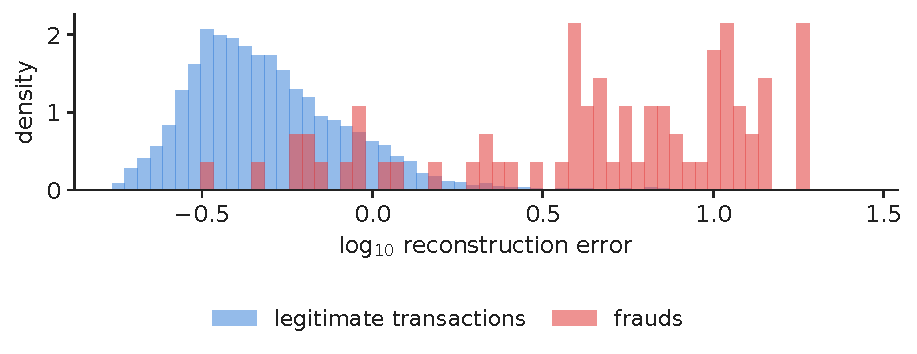
\includegraphics[width=\textwidth,height=0.550\textheight,keepaspectratio]{charts/en/ae_error_dist.pdf}\end{center}\vspace{-3mm}
\chartsource{Source: ULB Machine Learning Group and Worldline, credit-card transactions (OpenML 1597). Data: own estimates; two days of September 2013; test = last 20\,\% of the time span.}
\vspace{0.5mm}
\begin{itemize}\setlength{\itemsep}{0pt}
  \item \textbf{Separation}: the median error of a fraud is 12.7 times that of a legitimate transaction (test part).
  \item \textbf{Overlap}: many frauds still look normal to the autoencoder
    \begin{itemize}\setlength{\itemsep}{0pt}
      \item They sit in the bulk of the legitimate distribution.
    \end{itemize}
\end{itemize}
\par\vfill\noindent{\scriptsize\color{FooterGray}}\hfill\qlink{NN\_L8\_ae\_error\_dist}{Quantlets/L8/NN_L8_ae_error_dist}\par\vspace{0.5mm}
\end{frame}

\begin{frame}{Autoencoder without labels compared with a supervised classifier}
\small
\begin{center}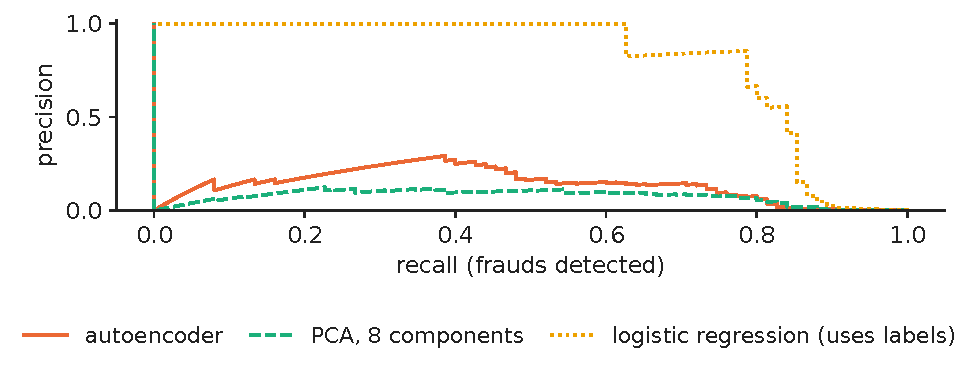
\includegraphics[width=\textwidth,height=0.458\textheight,keepaspectratio]{charts/en/ae_pr.pdf}\end{center}\vspace{-3mm}
\chartsource{Source: ULB Machine Learning Group and Worldline, credit-card transactions (OpenML 1597). Data: own estimates; two days of September 2013; test = last 20\,\% of the time span.}
\vspace{0.5mm}
\begin{itemize}\setlength{\itemsep}{0pt}
  \item \textbf{PR-AUC on the test part}: autoencoder 14.2\,\% (sd 2.9 over 3 seeds), PCA 7.6\,\%, logistic regression with labels 80.4\,\%
    \begin{itemize}\setlength{\itemsep}{0pt}
      \item A random score: 0.131\,\%.
    \end{itemize}
  \item \textbf{ROC-AUC} is high for all three (94.4, 95.3, 98.2\,\%): with 1 fraud in 700 it hides the difference that PR-AUC shows.
\end{itemize}
\par\vfill\noindent{\scriptsize\color{FooterGray}}\hfill\qlink{NN\_L8\_ae\_pr}{Quantlets/L8/NN_L8_ae_pr}\par\vspace{0.5mm}
\end{frame}

\begin{frame}{Bottleneck size and anomaly detection}
\small
\begin{center}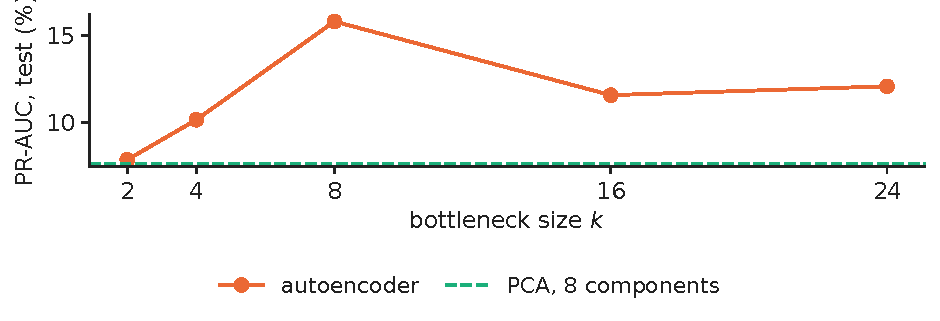
\includegraphics[width=\textwidth,height=0.395\textheight,keepaspectratio]{charts/en/ae_bottleneck.pdf}\end{center}\vspace{-3mm}
\chartsource{Source: ULB Machine Learning Group and Worldline, credit-card transactions (OpenML 1597). Data: own estimates; two days of September 2013; test = last 20\,\% of the time span.}
\vspace{0.5mm}
\begin{itemize}\setlength{\itemsep}{0pt}
  \item \textbf{PR-AUC by bottleneck size}: 7.8\,\% with $k=2$, 15.8\,\% with $k=8$, 12.1\,\% with $k=24$ (mean of 2 seeds)
    \begin{itemize}\setlength{\itemsep}{0pt}
      \item Best $k$ = 8.
    \end{itemize}
  \item \textbf{Too narrow}: even normal payments are rebuilt badly
    \begin{itemize}\setlength{\itemsep}{0pt}
      \item \textbf{too wide}: the network learns to copy frauds as well.
    \end{itemize}
\end{itemize}
\par\vfill\manager{choose $k$ on a validation period, never on the frauds you will report on.}\par\vspace{0.5mm}
\par\vfill\noindent{\scriptsize\color{FooterGray}}\hfill\qlink{NN\_L8\_ae\_bottleneck}{Quantlets/L8/NN_L8_ae_bottleneck}\par\vspace{0.5mm}
\end{frame}

\begin{frame}{Frauds found among the top 0.1\,\% of scores}
\footnotesize
\begin{columns}[T,onlytextwidth]
\begin{column}{0.52\textwidth}
{\scriptsize\renewcommand{\arraystretch}{1.3}\setlength{\tabcolsep}{4pt}
\begin{tabular}{@{}lrr@{}}\toprule
Detector & Frauds found & Share of frauds \\ \midrule
Autoencoder (no labels) & 8 & 10.7\,\% \\
PCA, 8 components (no labels) & 0 & 0.0\,\% \\
Logistic regression (labels) & 48 & 64.0\,\% \\
\bottomrule\end{tabular}}
\end{column}
\begin{column}{0.45\textwidth}
\begin{itemize}\setlength{\itemsep}{4pt}
  \item \textbf{Alert budget}
    \begin{itemize}\setlength{\itemsep}{0pt}
      \item 0.1\,\% of the test transactions = 57 alerts to review
    \end{itemize}
  \item \textbf{Reading}
    \begin{itemize}\setlength{\itemsep}{0pt}
      \item Labels are worth a lot: supervised learning wins whenever confirmed frauds exist
      \item The autoencoder is the detector of the unknown, a complement, not a replacement
    \end{itemize}
\end{itemize}
\end{column}
\end{columns}
\par\vfill\manager{run both: the classifier for known fraud patterns, the autoencoder to surface new ones for investigators to label.}\par\vspace{0.5mm}
\par\vfill\noindent{\scriptsize\color{FooterGray}(own computation, test part, weighted to the full data)}\hfill\tryit{notebook \S1}\par\vspace{0.5mm}
\end{frame}


\section{Variational autoencoders}

\begin{frame}{The VAE makes the autoencoder a probabilistic generator}
\footnotesize
\intuition{Instead of one code per input, the encoder outputs a distribution; the decoder learns to turn random codes into realistic data.}
\begin{columns}[T,onlytextwidth]
\begin{column}{0.58\textwidth}
\[ \log p_{\btheta}(\mathbf x)\ \ge\ \underbrace{\E_{q_{\phi}(\mathbf z\mid\mathbf x)}\big[\log p_{\btheta}(\mathbf x\mid\mathbf z)\big]}_{\text{reconstruction}}-\underbrace{\mathrm{KL}\big(q_{\phi}(\mathbf z\mid\mathbf x)\,\|\,p(\mathbf z)\big)}_{\text{regulariser}} \]{\footnotesize\begin{itemize}\setlength{\itemsep}{0pt}
  \item \textbf{\txtwhere}
    \begin{itemize}\setlength{\itemsep}{0pt}
      \item Right-hand side = evidence lower bound (ELBO)
      \item $q_\phi(\mathbf z\mid\mathbf x)=\mathcal N(\boldsymbol\mu_\phi(\mathbf x),\operatorname{diag}\boldsymbol\sigma^2_\phi(\mathbf x))$ = encoder
      \item $p_{\btheta}(\mathbf x\mid\mathbf z)$ = decoder
      \item $p(\mathbf z)=\mathcal N(0,I)$ = prior
      \item The second term is the Kullback--Leibler divergence (KL).
    \end{itemize}
\end{itemize}\par}
\end{column}
\begin{column}{0.39\textwidth}
\begin{itemize}\setlength{\itemsep}{3pt}
  \item \textbf{Why a bound}
    \begin{itemize}\setlength{\itemsep}{0pt}
      \item $\log p(\mathbf x)=\text{ELBO}+\mathrm{KL}\big(q(\mathbf z\mid\mathbf x)\|p(\mathbf z\mid\mathbf x)\big)$
      \item The gap is the error of the encoder; derivation in Appendix A
    \end{itemize}
  \item \textbf{Closed-form KL}
    \begin{itemize}\setlength{\itemsep}{0pt}
      \item $\mathrm{KL}=\tfrac12\sum_{j=1}^{k}\big(\mu_j^2+\sigma_j^2-\log\sigma_j^2-1\big)$
    \end{itemize}
\end{itemize}
\end{column}
\end{columns}
\par\vfill\manager{the KL term is what makes random codes meaningful: it packs all inputs around the origin of the latent space.}\par\vspace{0.5mm}
\par\vfill\noindent{\scriptsize\color{FooterGray}(Kingma \& Welling, 2014; Bishop \& Bishop, 2024, sec.\ 19.2)}\hfill\tryit{notebook \S2}\par\vspace{0.5mm}
\end{frame}

\begin{frame}{The reparameterisation trick}
\footnotesize
\intuition{Sampling is not differentiable, but a shifted and scaled standard normal is.}
\begin{columns}[T,onlytextwidth]
\begin{column}{0.58\textwidth}
\[ \mathbf z=\boldsymbol\mu_\phi(\mathbf x)+\boldsymbol\sigma_\phi(\mathbf x)\odot\boldsymbol\varepsilon,\qquad \boldsymbol\varepsilon\sim\mathcal N(0,I) \]\[ \nabla_\phi\,\E_{q_\phi}[h(\mathbf z)]=\E_{\boldsymbol\varepsilon}\big[\nabla_\phi\,h(\boldsymbol\mu_\phi+\boldsymbol\sigma_\phi\odot\boldsymbol\varepsilon)\big] \]{\footnotesize\begin{itemize}\setlength{\itemsep}{0pt}
  \item \textbf{\txtwhere}
    \begin{itemize}\setlength{\itemsep}{0pt}
      \item $\odot$ = element-wise product
      \item The randomness sits in $\boldsymbol\varepsilon$, which does not depend on $\phi$
      \item One draw of $\boldsymbol\varepsilon$ per image and step is enough in practice.
    \end{itemize}
\end{itemize}\par}
\end{column}
\begin{column}{0.39\textwidth}
\begin{itemize}\setlength{\itemsep}{3pt}
  \item \textbf{Our VAE on Fashion-MNIST}
    \begin{itemize}\setlength{\itemsep}{0pt}
      \item 28 $\times$ 28 grey images of 10 kinds of clothing, a drop-in for the MNIST digits
      \item 60\,000 training, 10\,000 test images; Bernoulli decoder (binary cross-entropy)
    \end{itemize}
  \item \textbf{Size}
    \begin{itemize}\setlength{\itemsep}{0pt}
      \item 784 $\to$ 400 $\to$ 200 $\to$ $k$; 798\,816 parameters for $k=16$; 20 epochs
    \end{itemize}
\end{itemize}
\end{column}
\end{columns}
\par\vfill\manager{the same trick drives every model that samples inside the network: VAEs, dropout as inference, stochastic policies.}\par\vspace{0.5mm}
\par\vfill\noindent{\scriptsize\color{FooterGray}(Kingma \& Welling, 2014; Xiao et al., 2017)}\hfill\tryit{notebook \S2}\par\vspace{0.5mm}
\end{frame}

\begin{frame}{A two-dimensional latent space separates the product types}
\small
\begin{center}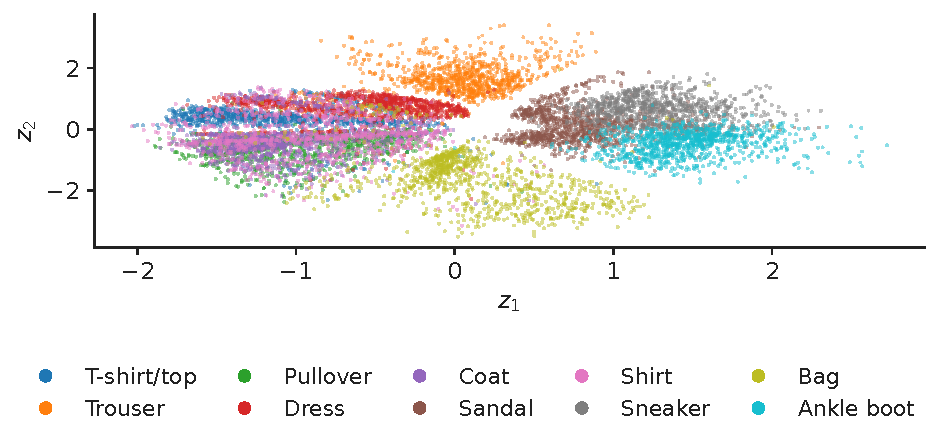
\includegraphics[width=\textwidth,height=0.580\textheight,keepaspectratio]{charts/en/vae_latent.pdf}\end{center}\vspace{-3mm}
\chartsource{Source: Fashion-MNIST, Zalando Research (Xiao et al., 2017). Data: own estimates; 60,000 training and 10,000 test images.}
\vspace{0.5mm}
\begin{itemize}\setlength{\itemsep}{0pt}
  \item \textbf{No labels used}: the VAE never saw the classes, yet shoes, bags and garments occupy separate regions.
  \item \textbf{Measured}: a 15-nearest-neighbour classifier on the two latent means reaches 71.7\,\% accuracy (5-fold, test images).
\end{itemize}
\par\vfill\noindent{\scriptsize\color{FooterGray}}\hfill\qlink{NN\_L8\_vae\_latent}{Quantlets/L8/NN_L8_vae_latent}\par\vspace{0.5mm}
\end{frame}

\begin{frame}{Quality of VAE reconstructions and generated samples}
\small
\begin{center}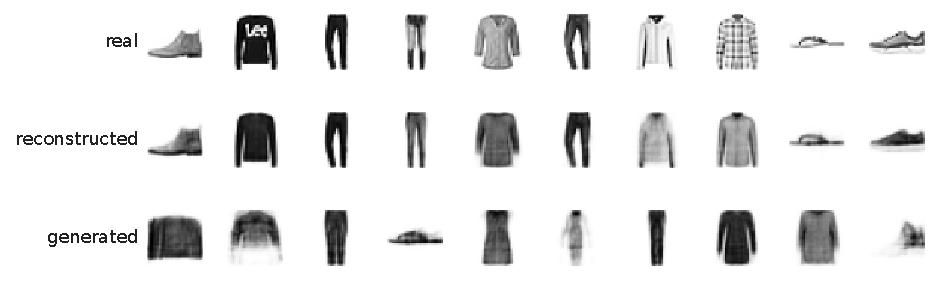
\includegraphics[width=\textwidth,height=0.480\textheight,keepaspectratio]{charts/en/vae_samples.pdf}\end{center}\vspace{-3mm}
\chartsource{Source: Fashion-MNIST, Zalando Research (Xiao et al., 2017). Data: own estimates; 60,000 training and 10,000 test images.}
\vspace{0.5mm}
\begin{itemize}\setlength{\itemsep}{0pt}
  \item \textbf{Rows}: real test images
    \begin{itemize}\setlength{\itemsep}{0pt}
      \item Their reconstructions through a 16-dimensional code
      \item New images decoded from random codes $\mathbf z\sim\mathcal N(0,I)$.
    \end{itemize}
  \item \textbf{Blur} comes from the Gaussian posterior and the pixel-wise loss: the decoder averages over plausible details.
\end{itemize}
\par\vfill\noindent{\scriptsize\color{FooterGray}}\hfill\qlink{NN\_L8\_vae\_samples}{Quantlets/L8/NN_L8_vae_samples}\par\vspace{0.5mm}
\end{frame}

\begin{frame}{Trade-off between reconstruction and the KL penalty during training}
\small
\begin{center}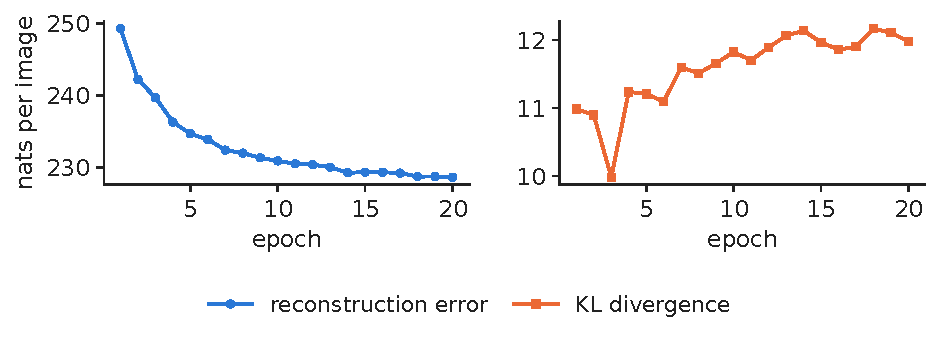
\includegraphics[width=\textwidth,height=0.480\textheight,keepaspectratio]{charts/en/vae_elbo.pdf}\end{center}\vspace{-3mm}
\chartsource{Source: Fashion-MNIST, Zalando Research (Xiao et al., 2017). Data: own estimates; 60,000 training and 10,000 test images.}
\vspace{0.5mm}
\begin{itemize}\setlength{\itemsep}{0pt}
  \item \textbf{Test, $k=16$, last epoch}: reconstruction 228.6 nats per image, KL 12.0 nats
    \begin{itemize}\setlength{\itemsep}{0pt}
      \item ELBO \ensuremath{-}240.6 nats.
    \end{itemize}
  \item \textbf{The KL rises} while the error falls: the encoder spends more information on each image as it learns.
\end{itemize}
\par\vfill\noindent{\scriptsize\color{FooterGray}(own computation, seed 1)}\hfill\qlink{NN\_L8\_vae\_elbo}{Quantlets/L8/NN_L8_vae_elbo}\par\vspace{0.5mm}
\end{frame}

\begin{frame}{$\beta$-VAE: reconstruction quality and latent-space structure}
\footnotesize
\begin{columns}[T,onlytextwidth]
\begin{column}{0.50\textwidth}
\[ \loss_\beta=-\E_{q}[\log p(\mathbf x\mid\mathbf z)]+\beta\,\mathrm{KL}\big(q(\mathbf z\mid\mathbf x)\|p(\mathbf z)\big) \]{\scriptsize\renewcommand{\arraystretch}{1.3}\setlength{\tabcolsep}{4pt}
\begin{tabular}{@{}lrrr@{}}\toprule
$\beta$ & Reconstruction & KL & Active dims \\ \midrule
0.5 & 222.5 & 17.8 & 9 \\
1.0 & 228.6 & 12.0 & 6 \\
4.0 & 242.5 & 6.4 & 4 \\
\bottomrule\end{tabular}}
\end{column}
\begin{column}{0.47\textwidth}
\begin{itemize}\setlength{\itemsep}{4pt}
  \item \textbf{Larger $\beta$}
    \begin{itemize}\setlength{\itemsep}{0pt}
      \item Fewer active latent dimensions (KL per dimension $>0.05$): from 9 to 4 of 16
      \item Worse reconstruction, smoother and more disentangled codes
    \end{itemize}
  \item \textbf{Smaller $\beta$}
    \begin{itemize}\setlength{\itemsep}{0pt}
      \item Closer to a plain autoencoder: good copies, poor samples
    \end{itemize}
\end{itemize}
\end{column}
\end{columns}
\par\vfill\manager{for scenario generation prefer a tidy latent space ($\beta\ge1$)
    \begin{itemize}\setlength{\itemsep}{0pt}
      \item For compression prefer reconstruction ($\beta<1$).
    \end{itemize}}\par\vspace{0.5mm}
\par\vfill\noindent{\scriptsize\color{FooterGray}(Higgins et al., 2017; own computation, test images, 20 epochs)}\hfill\tryit{notebook \S2}\par\vspace{0.5mm}
\end{frame}


\section{Generative adversarial networks}

\begin{frame}{Generative adversarial networks: generator and discriminator}
\footnotesize
\intuition{The generator turns noise into fake data; the discriminator tries to tell fake from real; each improves against the other.}
\begin{columns}[T,onlytextwidth]
\begin{column}{0.58\textwidth}
\[ \min_{G}\max_{D}\ \E_{\mathbf x\sim p_{data}}\big[\log D(\mathbf x)\big]+\E_{\mathbf z\sim p(\mathbf z)}\big[\log\big(1-D(G(\mathbf z))\big)\big] \]\[ D^{*}(\mathbf x)=\frac{p_{data}(\mathbf x)}{p_{data}(\mathbf x)+p_G(\mathbf x)}\ \Rightarrow\ \text{value}=-\log4+2\,\mathrm{JS}(p_{data}\|p_G) \]{\footnotesize\begin{itemize}\setlength{\itemsep}{0pt}
  \item \textbf{\txtwhere}
    \begin{itemize}\setlength{\itemsep}{0pt}
      \item $G$ = generator network, $D$ = discriminator (probability that $\mathbf x$ is real)
      \item $p_G$ = distribution of $G(\mathbf z)$
      \item Jensen--Shannon divergence (JS), zero only when $p_G=p_{data}$.
    \end{itemize}
\end{itemize}\par}
\end{column}
\begin{column}{0.39\textwidth}
\begin{itemize}\setlength{\itemsep}{3pt}
  \item \textbf{At equilibrium}
    \begin{itemize}\setlength{\itemsep}{0pt}
      \item $D^{*}=1/2$ everywhere: the detective can only guess; discriminator loss $2\log 2$
    \end{itemize}
  \item \textbf{No likelihood}
    \begin{itemize}\setlength{\itemsep}{0pt}
      \item A GAN never writes down $p_G$; it only learns to sample from it
    \end{itemize}
\end{itemize}
\end{column}
\end{columns}
\par\vfill\manager{GANs are judged by what their samples get right (tails, dependence), not by a likelihood number.}\par\vspace{0.5mm}
\par\vfill\noindent{\scriptsize\color{FooterGray}(Goodfellow et al., 2014; Bishop \& Bishop, 2024, ch.\ 17)}\hfill\tryit{notebook \S3}\par\vspace{0.5mm}
\end{frame}

\begin{frame}{Training a GAN: alternate steps and the non-saturating loss}
\footnotesize
\intuition{Each step updates the detective on a batch of real and fake data, then the forger on fresh noise.}
\begin{columns}[T,onlytextwidth]
\begin{column}{0.58\textwidth}
\[ \loss_D=-\tfrac1m\sum_{i}\big[\log D(\mathbf x_i)+\log(1-D(G(\mathbf z_i)))\big] \]\[ \loss_G=-\tfrac1m\sum_{i}\log D(G(\mathbf z_i))\quad\text{(non-saturating)} \]{\footnotesize\begin{itemize}\setlength{\itemsep}{0pt}
  \item \textbf{\txtwhere}
    \begin{itemize}\setlength{\itemsep}{0pt}
      \item $m=256$ days per batch
      \item $\mathbf z\in\R^8$ standard normal
      \item $\loss_G$ replaces $\log(1-D(G))$, whose gradient vanishes when $D$ wins early
      \item Adam with learning rate $2\cdot10^{-4}$, $\beta_1=0.5$.
    \end{itemize}
\end{itemize}\par}
\end{column}
\begin{column}{0.39\textwidth}
\begin{itemize}\setlength{\itemsep}{3pt}
  \item \textbf{Our GAN}
    \begin{itemize}\setlength{\itemsep}{0pt}
      \item S\&P 500 daily log returns 4 Jan 2005 to 2019, 3\,774 days, standardised
      \item Generator 4\,801 and discriminator 4\,353 parameters; 6\,000 steps, 3 seeds
    \end{itemize}
\end{itemize}
\end{column}
\end{columns}
\par\vfill\manager{watch both losses: a discriminator loss stuck at zero means the generator has stopped learning.}\par\vspace{0.5mm}
\par\vfill\noindent{\scriptsize\color{FooterGray}(Goodfellow et al., 2014)}\hfill\tryit{notebook \S3}\par\vspace{0.5mm}
\end{frame}

\begin{frame}{The two losses settle near the equilibrium values}
\small
\begin{center}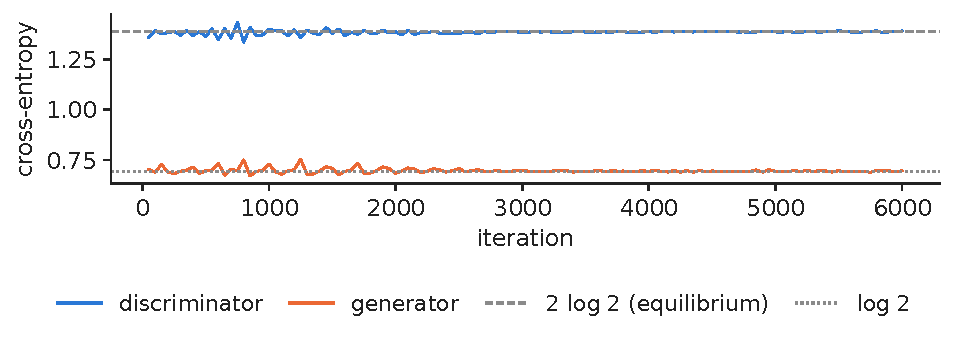
\includegraphics[width=\textwidth,height=0.500\textheight,keepaspectratio]{charts/en/gan_losses.pdf}\end{center}\vspace{-3mm}
\chartsource{Source: Yahoo Finance, daily quotes. Data: own estimates; S\&P 500 4 Jan 2005 to 31 Dec 2019, trading days.}
\vspace{0.5mm}
\begin{itemize}\setlength{\itemsep}{0pt}
  \item \textbf{Equilibrium}: the discriminator loss hovers around $2\log2$ and the generator loss around $\log 2$, the values of $D^{*}=1/2$.
  \item \textbf{No convergence proof}: gradient play can cycle
    \begin{itemize}\setlength{\itemsep}{0pt}
      \item The loss curves do not measure sample quality.
    \end{itemize}
\end{itemize}
\par\vfill\noindent{\scriptsize\color{FooterGray}}\hfill\qlink{NN\_L8\_gan\_losses}{Quantlets/L8/NN_L8_gan_losses}\par\vspace{0.5mm}
\end{frame}

\begin{frame}{The GAN reproduces the fat tails missed by the Gaussian model}
\small
\begin{center}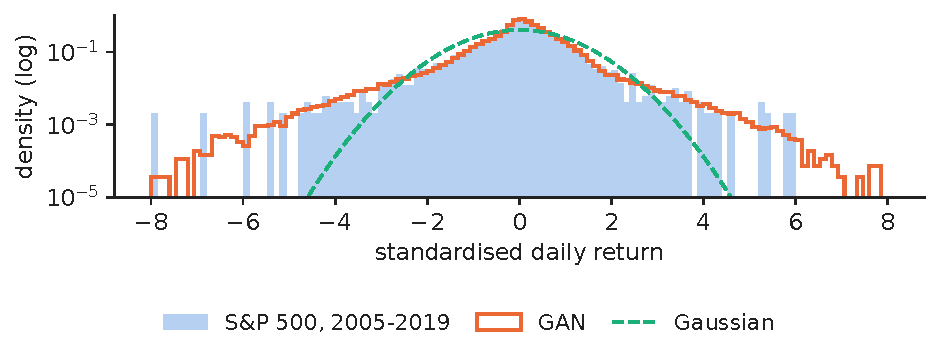
\includegraphics[width=\textwidth,height=0.520\textheight,keepaspectratio]{charts/en/gan_density.pdf}\end{center}\vspace{-3mm}
\chartsource{Source: Yahoo Finance, daily quotes. Data: own estimates; S\&P 500 4 Jan 2005 to 31 Dec 2019, trading days.}
\vspace{0.5mm}
\begin{itemize}\setlength{\itemsep}{0pt}
  \item \textbf{Excess kurtosis}: real 11.86, GAN 6.65 (sd 0.48 over 3 seeds), Gaussian 0.
  \item \textbf{Kolmogorov--Smirnov distance} to the real returns: GAN 0.030, fitted Gaussian 0.115.
\end{itemize}
\par\vfill\noindent{\scriptsize\color{FooterGray}(Cont, 2001)}\hfill\qlink{NN\_L8\_gan\_density}{Quantlets/L8/NN_L8_gan_density}\par\vspace{0.5mm}
\end{frame}

\begin{frame}{A risk check: 1\,\% Value-at-Risk on the years after training}
\footnotesize
\begin{columns}[T,onlytextwidth]
\begin{column}{0.52\textwidth}
\[ \mathrm{VaR}_{0.01}=-q_{0.01}(r),\qquad \hat\pi=\frac{1}{T}\sum_{t=1}^{T}\mathbf 1\{r_t<q_{0.01}\} \]{\scriptsize\renewcommand{\arraystretch}{1.3}\setlength{\tabcolsep}{4pt}
\begin{tabular}{@{}lrr@{}}\toprule
Method (fitted 2005--2019) & 1\,\% quantile & Exceedances \\ \midrule
Historical simulation & \ensuremath{-}3.48\,\% & 1.11\,\% \\
GAN samples (3 seeds) & \ensuremath{-}3.61\,\% & 0.95\,\% \\
Gaussian & \ensuremath{-}2.67\,\% & 2.39\,\% \\
\bottomrule\end{tabular}}
\end{column}
\begin{column}{0.45\textwidth}
\begin{itemize}\setlength{\itemsep}{4pt}
  \item \textbf{Test period}
    \begin{itemize}\setlength{\itemsep}{0pt}
      \item 2 Jan 2020 to 30 Oct 2026, 1\,717 days; a correct 1\,\% VaR is exceeded on about 17 days
    \end{itemize}
  \item \textbf{Reading}
    \begin{itemize}\setlength{\itemsep}{0pt}
      \item The GAN quantile is as good as historical simulation; the Gaussian is exceeded 2.39\,\% of the days
      \item Unconditional quantiles only: no model here reacts to volatility
      \item The expected shortfall (ES), the mean loss beyond the VaR, depends on the same tail
    \end{itemize}
\end{itemize}
\end{column}
\end{columns}
\par\vfill\manager{a generator is only as good as the risk number it reproduces: backtest it like any VaR model (Kupiec, 1995).}\par\vspace{0.5mm}
\par\vfill\noindent{\scriptsize\color{FooterGray}(own computation)}\hfill\tryit{notebook \S3}\par\vspace{0.5mm}
\end{frame}

\begin{frame}{A GAN on single days cannot learn volatility clustering}
\small
\begin{center}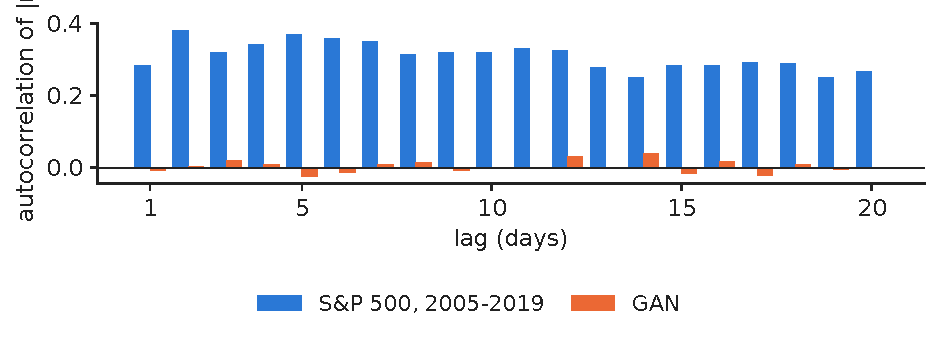
\includegraphics[width=\textwidth,height=0.480\textheight,keepaspectratio]{charts/en/gan_acf.pdf}\end{center}\vspace{-3mm}
\chartsource{Source: Yahoo Finance, daily quotes. Data: own estimates; S\&P 500 4 Jan 2005 to 31 Dec 2019, trading days.}
\vspace{0.5mm}
\begin{itemize}\setlength{\itemsep}{0pt}
  \item \textbf{Real returns}: the autocorrelation of $|r_t|$ is 0.28 at lag 1 and still 0.27 at lag 20: calm and turbulent periods cluster.
  \item \textbf{GAN samples} are independent draws (\ensuremath{-}0.01 at lag 1): the right marginal, the wrong dynamics
    \begin{itemize}\setlength{\itemsep}{0pt}
      \item Sequence models (TimeGAN, Quant GANs) generate whole paths.
    \end{itemize}
\end{itemize}
\par\vfill\noindent{\scriptsize\color{FooterGray}(Cont, 2001; Yoon et al., 2019; Wiese et al., 2020)}\hfill\qlink{NN\_L8\_gan\_acf}{Quantlets/L8/NN_L8_gan_acf}\par\vspace{0.5mm}
\end{frame}

\begin{frame}{Mode collapse and the Wasserstein GAN}
\footnotesize
\intuition{A generator can win by producing a few convincing samples; the Wasserstein distance gives useful gradients even when the supports do not overlap.}
\begin{columns}[T,onlytextwidth]
\begin{column}{0.58\textwidth}
\[ W_1(p_{data},p_G)=\sup_{\|f\|_{L}\le1}\ \E_{p_{data}}[f(\mathbf x)]-\E_{p_G}[f(\mathbf x)] \]{\footnotesize\begin{itemize}\setlength{\itemsep}{0pt}
  \item \textbf{\txtwhere}
    \begin{itemize}\setlength{\itemsep}{0pt}
      \item $f$ = critic network, constrained to be 1-Lipschitz (weight clipping or a gradient penalty)
      \item The generator minimises $W_1$: the Wasserstein GAN (WGAN).
    \end{itemize}
\end{itemize}\par}
\end{column}
\begin{column}{0.39\textwidth}
\begin{itemize}\setlength{\itemsep}{3pt}
  \item \textbf{Mode collapse}
    \begin{itemize}\setlength{\itemsep}{0pt}
      \item The generator maps all $\mathbf z$ to one region: e.g.\ only calm days, never crashes
    \end{itemize}
  \item \textbf{Checks}
    \begin{itemize}\setlength{\itemsep}{0pt}
      \item Compare tail quantiles, the share of extreme days and the spread of samples with the real data
    \end{itemize}
\end{itemize}
\end{column}
\end{columns}
\par\vfill\manager{a stress-test generator that has collapsed onto calm days is worse than no generator.}\par\vspace{0.5mm}
\par\vfill\noindent{\scriptsize\color{FooterGray}(Arjovsky, Chintala \& Bottou, 2017)}\par\vspace{0.5mm}
\end{frame}


\section{Diffusion models}

\begin{frame}{Diffusion models: forward noising and reverse denoising}
\footnotesize
\intuition{Adding a little Gaussian noise many times turns any data into pure noise; a network learns each small reverse step.}
\begin{columns}[T,onlytextwidth]
\begin{column}{0.58\textwidth}
\[ q(\mathbf x_t\mid\mathbf x_{t-1})=\mathcal N\big(\sqrt{1-\beta_t}\,\mathbf x_{t-1},\ \beta_tI\big) \]\[ q(\mathbf x_t\mid\mathbf x_0)=\mathcal N\big(\sqrt{\bar\alpha_t}\,\mathbf x_0,\ (1-\bar\alpha_t)I\big),\quad \bar\alpha_t=\prod_{s=1}^{t}(1-\beta_s) \]{\footnotesize\begin{itemize}\setlength{\itemsep}{0pt}
  \item \textbf{\txtwhere}
    \begin{itemize}\setlength{\itemsep}{0pt}
      \item $\mathbf x_0$ = a real observation (here a standardised yield curve)
      \item $\beta_t$ = noise schedule, linear from $10^{-4}$ to 0.02 over $T$ = 200 steps
      \item $\bar\alpha_T\approx0$, so $\mathbf x_T$ is almost standard normal.
    \end{itemize}
\end{itemize}\par}
\end{column}
\begin{column}{0.39\textwidth}
\begin{itemize}\setlength{\itemsep}{3pt}
  \item \textbf{Closed form}
    \begin{itemize}\setlength{\itemsep}{0pt}
      \item Any step $t$ is reached in one draw: $\mathbf x_t=\sqrt{\bar\alpha_t}\mathbf x_0+\sqrt{1-\bar\alpha_t}\,\boldsymbol\varepsilon$
    \end{itemize}
  \item \textbf{No parameters}
    \begin{itemize}\setlength{\itemsep}{0pt}
      \item The forward process is fixed; only the reverse process is learnt
    \end{itemize}
\end{itemize}
\end{column}
\end{columns}
\par\vfill\manager{diffusion turns generation into many small regression problems, which is why it trains stably.}\par\vspace{0.5mm}
\par\vfill\noindent{\scriptsize\color{FooterGray}(Sohl-Dickstein et al., 2015; Ho, Jain \& Abbeel, 2020)}\hfill\tryit{notebook \S4}\par\vspace{0.5mm}
\end{frame}

\begin{frame}{The forward process on a real yield curve}
\small
\begin{center}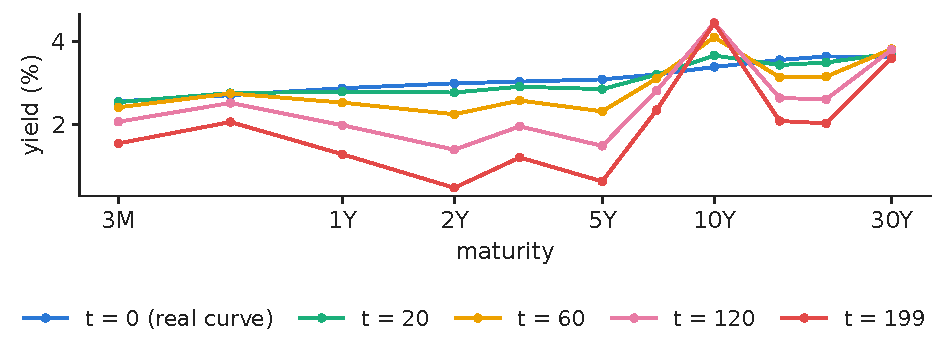
\includegraphics[width=\textwidth,height=0.520\textheight,keepaspectratio]{charts/en/diffusion_forward.pdf}\end{center}\vspace{-3mm}
\chartsource{Source: European Central Bank, euro area AAA yield curve. Data: curve of 30 Oct 2026; noise schedule of the lecture (mechanism).}
\vspace{0.5mm}
\begin{itemize}\setlength{\itemsep}{0pt}
  \item \textbf{Curve of 30 Oct 2026}, 11 maturities from 3 months to 30 years
    \begin{itemize}\setlength{\itemsep}{0pt}
      \item By $t=199$ the shape is gone and only noise remains.
    \end{itemize}
  \item \textbf{The network} must learn to walk back from right to left, one small step at a time.
\end{itemize}
\par\vfill\noindent{\scriptsize\color{FooterGray}(mechanism shown on real data; one draw of the noise)}\hfill\qlink{NN\_L8\_diffusion\_forward}{Quantlets/L8/NN_L8_diffusion_forward}\par\vspace{0.5mm}
\end{frame}

\begin{frame}{Learning to denoise: predict the noise that was added}
\footnotesize
\intuition{The network sees a noisy curve and the step $t$, and guesses the noise; subtracting the guess, step by step, gives a new curve.}
\begin{columns}[T,onlytextwidth]
\begin{column}{0.58\textwidth}
\[ \loss(\btheta)=\E_{t,\mathbf x_0,\boldsymbol\varepsilon}\Big\|\boldsymbol\varepsilon-\boldsymbol\varepsilon_{\btheta}\big(\sqrt{\bar\alpha_t}\mathbf x_0+\sqrt{1-\bar\alpha_t}\,\boldsymbol\varepsilon,\ t\big)\Big\|^2 \]\[ \mathbf x_{t-1}=\frac{1}{\sqrt{\alpha_t}}\Big(\mathbf x_t-\frac{\beta_t}{\sqrt{1-\bar\alpha_t}}\boldsymbol\varepsilon_{\btheta}(\mathbf x_t,t)\Big)+\sqrt{\beta_t}\,\mathbf u,\ \ \mathbf u\sim\mathcal N(0,I) \]{\footnotesize\begin{itemize}\setlength{\itemsep}{0pt}
  \item \textbf{\txtwhere}
    \begin{itemize}\setlength{\itemsep}{0pt}
      \item $\boldsymbol\varepsilon_{\btheta}$ = denoiser network
      \item $\alpha_t=1-\beta_t$
      \item $t$ uniform on $\{1,\dots,T\}$
      \item The loss is a simplified, reweighted ELBO.
    \end{itemize}
\end{itemize}\par}
\end{column}
\begin{column}{0.39\textwidth}
\begin{itemize}\setlength{\itemsep}{3pt}
  \item \textbf{Our denoiser}
    \begin{itemize}\setlength{\itemsep}{0pt}
      \item MLP with 3 hidden layers of 256 and a sinusoidal embedding of $t$: 145\,675 parameters
      \item 12\,000 steps of 512 curves; 5,000 curves sampled per seed
    \end{itemize}
  \item \textbf{Data}
    \begin{itemize}\setlength{\itemsep}{0pt}
      \item 5\,664 daily curves of the European Central Bank, 6 Sep 2004 to 30 Oct 2026
    \end{itemize}
\end{itemize}
\end{column}
\end{columns}
\par\vfill\manager{the same loss, with images and a text condition, runs the image generators you know
    \begin{itemize}\setlength{\itemsep}{0pt}
      \item Here it generates interest-rate scenarios.
    \end{itemize}}\par\vspace{0.5mm}
\par\vfill\noindent{\scriptsize\color{FooterGray}(Ho, Jain \& Abbeel, 2020; Bishop \& Bishop, 2024, ch.\ 20)}\hfill\tryit{notebook \S4}\par\vspace{0.5mm}
\end{frame}

\begin{frame}{The two regimes of euro rates in diffusion and Gaussian samples}
\small
\begin{center}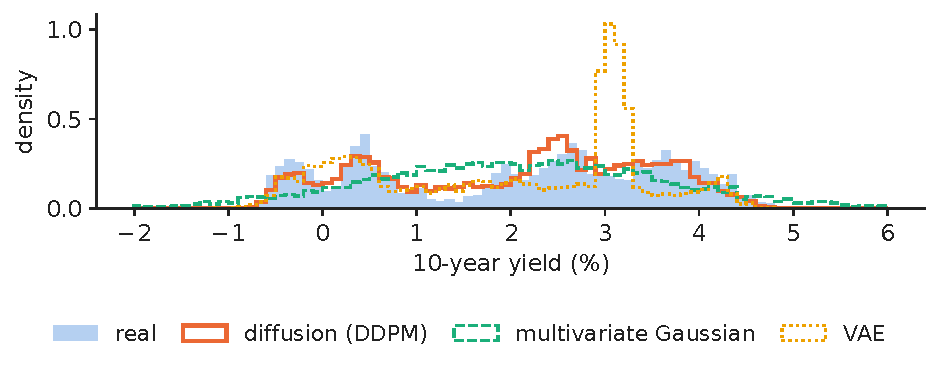
\includegraphics[width=\textwidth,height=0.520\textheight,keepaspectratio]{charts/en/yc_density.pdf}\end{center}\vspace{-3mm}
\chartsource{Source: European Central Bank, euro area AAA yield curve. Data: own estimates; 6 Sep 2004 to 30 Oct 2026, business days.}
\vspace{0.5mm}
\begin{itemize}\setlength{\itemsep}{0pt}
  \item \textbf{Real 10-year yield}: from \ensuremath{-}0.82\,\% to 4.78\,\%, negative on 13.8\,\% of the days: a low-rate and a normal-rate regime.
  \item \textbf{Wasserstein distance} of the generated 10-year yield to the real one: DDPM 0.149, VAE 0.191, Gaussian 0.325 percentage points.
\end{itemize}
\par\vfill\noindent{\scriptsize\color{FooterGray}}\hfill\qlink{NN\_L8\_yc\_density}{Quantlets/L8/NN_L8_yc_density}\par\vspace{0.5mm}
\end{frame}

\begin{frame}{Diffusion preserves the nonlinear co-movement of level and slope}
\small
\begin{center}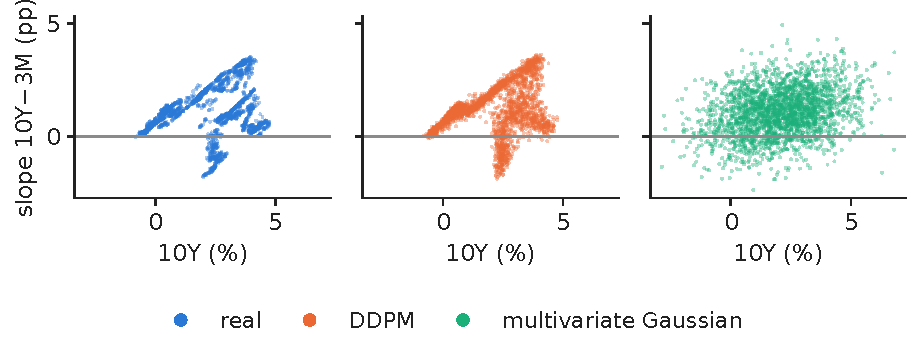
\includegraphics[width=\textwidth,height=0.500\textheight,keepaspectratio]{charts/en/yc_scatter.pdf}\end{center}\vspace{-3mm}
\chartsource{Source: European Central Bank, euro area AAA yield curve. Data: own estimates; 6 Sep 2004 to 30 Oct 2026, business days.}
\vspace{0.5mm}
\begin{itemize}\setlength{\itemsep}{0pt}
  \item \textbf{Inverted curves} (10 years below 3 months): 8.7\,\% of real days, 10.2\,\% of diffusion samples, 14.7\,\% of Gaussian samples.
  \item \textbf{Slope distance} (Wasserstein): DDPM 0.099, VAE 0.242, Gaussian 0.113.
\end{itemize}
\par\vfill\noindent{\scriptsize\color{FooterGray}}\hfill\qlink{NN\_L8\_yc\_scatter}{Quantlets/L8/NN_L8_yc_scatter}\par\vspace{0.5mm}
\end{frame}

\begin{frame}{A two-factor VAE of the curve rediscovers level and slope}
\small
\begin{center}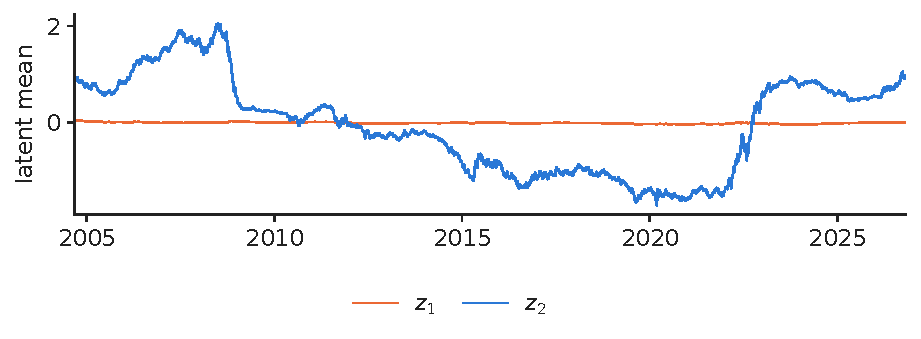
\includegraphics[width=\textwidth,height=0.480\textheight,keepaspectratio]{charts/en/yc_latent_time.pdf}\end{center}\vspace{-3mm}
\chartsource{Source: European Central Bank, euro area AAA yield curve. Data: own estimates; 6 Sep 2004 to 30 Oct 2026, business days.}
\vspace{0.5mm}
\begin{itemize}\setlength{\itemsep}{0pt}
  \item \textbf{Correlations} of the latent means with the level (mean of the 11 yields) and the slope (10 years minus 3 months): up to 0.99 and 0.66 in absolute value.
  \item \textbf{Interpretable compression}: the latent path tracks the 2014--2021 low-rate era and the 2022 tightening without being told.
\end{itemize}
\par\vfill\noindent{\scriptsize\color{FooterGray}(Svensson, 1994)}\hfill\qlink{NN\_L8\_yc\_latent\_time}{Quantlets/L8/NN_L8_yc_latent_time}\par\vspace{0.5mm}
\end{frame}


\section{Generative models in practice}

\begin{frame}{Evaluation criteria for synthetic financial data}
\footnotesize
\begin{columns}[T,onlytextwidth]
\begin{column}{0.49\textwidth}
\begin{itemize}\setlength{\itemsep}{5pt}
  \item \textbf{Fidelity}
    \begin{itemize}\setlength{\itemsep}{0pt}
      \item Marginals and tails (kurtosis, 1\,\% quantile), dependence across assets and over time (autocorrelation of $|r_t|$)
    \end{itemize}
  \item \textbf{Diversity}
    \begin{itemize}\setlength{\itemsep}{0pt}
      \item No mode collapse: the share of extreme days and regimes as in the data
    \end{itemize}
  \item \textbf{Utility}
    \begin{itemize}\setlength{\itemsep}{0pt}
      \item Train on synthetic, test on real (TSTR): a model fitted on synthetic data must work on real data
    \end{itemize}
\end{itemize}
\end{column}
\begin{column}{0.48\textwidth}
\begin{itemize}\setlength{\itemsep}{5pt}
  \item \textbf{Privacy}
    \begin{itemize}\setlength{\itemsep}{0pt}
      \item Generators can memorise records: check the distance of each sample to its nearest real record
    \end{itemize}
  \item \textbf{Our scorecard}
    \begin{itemize}\setlength{\itemsep}{0pt}
      \item GAN returns: tails right, clustering wrong
      \item DDPM curves: regimes and inversions right, Gaussian wrong
    \end{itemize}
\end{itemize}
\end{column}
\end{columns}
\par\vfill\manager{never use synthetic data for a decision before it passes the same backtests as the model it feeds.}\par\vspace{0.5mm}
\par\vfill\noindent{\scriptsize\color{FooterGray}(Cont, 2001; Yoon et al., 2019)}\par\vspace{0.5mm}
\end{frame}

\begin{frame}{Choosing a generative model}
\footnotesize
{\scriptsize\renewcommand{\arraystretch}{1.25}\setlength{\tabcolsep}{4pt}
\begin{tabular}{@{}p{0.22\textwidth}p{0.17\textwidth}p{0.17\textwidth}p{0.17\textwidth}p{0.17\textwidth}@{}}\toprule
Need & AE & VAE & GAN & DDPM \\ \midrule
Anomaly score & yes (error) & yes (ELBO) & indirect & yes (bound) \\
Sample quality & -- & blurry & sharp & best \\
Sampling speed & -- & one pass & one pass & 200 passes \\
Training stability & high & high & low & high \\
Latent factors & yes & yes, smooth & no inverse & no \\
\bottomrule\end{tabular}}
\vspace{2mm}
\begin{itemize}\setlength{\itemsep}{2pt}
  \item \textbf{Rule of thumb}: autoencoders to monitor, VAEs to compress and explore, diffusion to simulate faithfully, GAN models when sampling must be fast.
\end{itemize}
\par\vfill\noindent{\scriptsize\color{FooterGray}(Bishop \& Bishop, 2024, ch.\ 16--20)}\par\vspace{0.5mm}
\end{frame}


\section{Wrap-up}

\begin{frame}{Key takeaways}
\small
\begin{itemize}\setlength{\itemsep}{6pt}
  \item \textbf{Autoencoders} model ``normal'': on card fraud PR-AUC 14.2\,\% without labels, against 80.4\,\% for a classifier that uses labels.
  \item \textbf{VAEs} maximise the ELBO = reconstruction $-$ KL
    \begin{itemize}\setlength{\itemsep}{0pt}
      \item The reparameterisation trick makes them trainable
      \item $\beta$ trades detail for a tidy latent space.
    \end{itemize}
  \item \textbf{GANs} reproduce fat tails (kurtosis 6.65 vs 11.86 real) and a usable 1\,\% VaR, but not volatility clustering when trained on single days.
  \item \textbf{Diffusion} learns to undo noise
    \begin{itemize}\setlength{\itemsep}{0pt}
      \item On euro yield curves it keeps both rate regimes and the inversions that a Gaussian misses.
    \end{itemize}
\end{itemize}
\end{frame}

\begin{frame}{Research from our group: generative models for tail risk}
\footnotesize
\begin{itemize}\setlength{\itemsep}{5pt}
  \item \textbf{Large language models (LLM) as risk forecasters: LLM-VaR and LLM-ES} (Pele, Bolovăneanu, Lin, Ren, Ginavar, Spilak, Andrei, Toma, Lessmann \& Härdle, 2026): uses generative language models, prompted with return histories, to forecast Value-at-Risk and expected shortfall, evaluated with standard risk backtests.
  \item \textbf{Foundation models for tail risk} (Jheng, Tak, Găman, Mazurencu-Marinescu-Pele \& Pele, 2026): uses pretrained probabilistic forecasting models, which generate sample paths, without retraining and with conformal calibration, to forecast VaR and ES in Central and Eastern European markets.
  \item \textbf{Link with this lecture}: both treat a generator of scenarios as a risk model, and judge it by the backtests used on this lecture's GAN.
\end{itemize}
\vspace{1mm}{\scriptsize Findings as stated in the papers; the numbers on the other slides come from our own computations.}
\par\vfill\noindent{\scriptsize\color{FooterGray}(Bucharest University of Economic Studies; Romanian Academy, Institute for Economic Forecasting)}\par\vspace{0.5mm}
\end{frame}

\begin{frame}{Further reading and resources}
\small
\begin{columns}[T,onlytextwidth]
\begin{column}{0.52\textwidth}
\begin{itemize}\setlength{\itemsep}{4pt}
  \item \textbf{Bishop \& Bishop (2024)}, chapters 16--20: latent variables, GANs, flows, autoencoders, diffusion.
  \item \textbf{Lilian Weng's notes} on diffusion models: \href{https://lilianweng.github.io/posts/2021-07-11-diffusion-models/}{lilianweng.github.io}.
  \item \textbf{Ho et al.\ (2020)}, the DDPM paper, short and readable.
\end{itemize}
\end{column}
\begin{column}{0.45\textwidth}
\begin{itemize}\setlength{\itemsep}{4pt}
  \item \textbf{This course}: code, data, notebooks --- \href{https://github.com/danpele/NEURAL_BIZ}{github.com/danpele/NEURAL\_BIZ}.
  \item \textbf{Experiment yourself}: the notebook reproduces every chart and number of this lecture.
\end{itemize}
\end{column}
\end{columns}
\end{frame}

\begin{frame}{Quiz 1: autoencoder}
\small
\begin{itemize}
  \item Why is the fraud autoencoder trained on legitimate transactions only?
\end{itemize}
\vspace{2mm}
\begin{exampleblock}{Answer}
\begin{itemize}
  \item It must learn what ``normal'' looks like
    \begin{itemize}\setlength{\itemsep}{0pt}
      \item Frauds are then rebuilt badly and get a high score (median error 12.7 times larger).
    \end{itemize}
\end{itemize}
\end{exampleblock}
\end{frame}

\begin{frame}{Quiz 2: ELBO}
\small
\begin{itemize}
  \item Which two terms make up the ELBO, and what does each do?
\end{itemize}
\vspace{2mm}
\begin{exampleblock}{Answer}
\begin{itemize}
  \item Expected log-likelihood of the data given the code (reconstruction) minus the KL divergence of the encoder from the prior (keeps codes near $\mathcal N(0,I)$, so random codes decode to realistic data).
\end{itemize}
\end{exampleblock}
\end{frame}

\begin{frame}{Quiz 3: GAN equilibrium}
\small
\begin{itemize}
  \item What does the optimal discriminator output once the generator matches the data?
\end{itemize}
\vspace{2mm}
\begin{exampleblock}{Answer}
\begin{itemize}
  \item $D^{*}(\mathbf x)=1/2$ everywhere, because $p_{data}=p_G$
    \begin{itemize}\setlength{\itemsep}{0pt}
      \item Its loss is then $2\log2$.
    \end{itemize}
\end{itemize}
\end{exampleblock}
\end{frame}

\begin{frame}{Quiz 4: synthetic returns}
\small
\begin{itemize}
  \item Our GAN gets the tails of S\&P 500 returns right.
    \begin{itemize}\setlength{\itemsep}{0pt}
      \item Why is it still unfit for a volatility model?
    \end{itemize}
\end{itemize}
\vspace{2mm}
\begin{exampleblock}{Answer}
\begin{itemize}
  \item It draws days independently: the autocorrelation of $|r_t|$ is \ensuremath{-}0.01 instead of 0.28
    \begin{itemize}\setlength{\itemsep}{0pt}
      \item Volatility clustering needs a sequence generator.
    \end{itemize}
\end{itemize}
\end{exampleblock}
\end{frame}

\begin{frame}{Quiz 5: diffusion}
\small
\begin{itemize}
  \item What does the diffusion network predict during training?
\end{itemize}
\vspace{2mm}
\begin{exampleblock}{Answer}
\begin{itemize}
  \item The Gaussian noise $\boldsymbol\varepsilon$ that was added to $\mathbf x_0$ to obtain $\mathbf x_t$, given $\mathbf x_t$ and $t$
    \begin{itemize}\setlength{\itemsep}{0pt}
      \item Generation subtracts the predicted noise step by step.
    \end{itemize}
\end{itemize}
\end{exampleblock}
\end{frame}

\begin{frame}{References (1/2)}
\scriptsize
\begin{itemize}\setlength{\itemsep}{0pt}\scriptsize
\item Arjovsky, M., Chintala, S.\ \& Bottou, L.\ (2017). Wasserstein generative adversarial networks. \textit{Proceedings of ICML}, PMLR 70, 214--223. \href{https://arxiv.org/abs/1701.07875}{arXiv:1701.07875}
\item Bishop, C.\,M.\ \& Bishop, H.\ (2024). \textit{Deep Learning: Foundations and Concepts}, ch.\ 16--20. Springer. \href{https://doi.org/10.1007/978-3-031-45468-4}{doi:10.1007/978-3-031-45468-4}
\item Cont, R.\ (2001). Empirical properties of asset returns: stylized facts and statistical issues. \textit{Quantitative Finance}, 1(2), 223--236. \href{https://doi.org/10.1080/713665670}{doi:10.1080/713665670}
\item Dal Pozzolo, A., Caelen, O., Johnson, R.\,A.\ \& Bontempi, G.\ (2015). Calibrating probability with undersampling for unbalanced classification. \textit{IEEE Symposium Series on Computational Intelligence}, 159--166. \href{https://doi.org/10.1109/SSCI.2015.33}{doi:10.1109/SSCI.2015.33}
\item Goodfellow, I., Pouget-Abadie, J., Mirza, M., Xu, B., Warde-Farley, D., Ozair, S., Courville, A.\ \& Bengio, Y.\ (2014). Generative adversarial nets. \textit{Advances in Neural Information Processing Systems}, 27. \href{https://arxiv.org/abs/1406.2661}{arXiv:1406.2661}
\item Higgins, I., Matthey, L., Pal, A.\ et al.\ (2017). beta-VAE: Learning basic visual concepts with a constrained variational framework. \textit{International Conference on Learning Representations}. \href{https://openreview.net/forum?id=Sy2fzU9gl}{openreview.net}
\item Ho, J., Jain, A.\ \& Abbeel, P.\ (2020). Denoising diffusion probabilistic models. \textit{Advances in Neural Information Processing Systems}, 33. \href{https://arxiv.org/abs/2006.11239}{arXiv:2006.11239}
\item Jheng, S.-L., Tak, R., Găman, Ș., Mazurencu-Marinescu-Pele, M.\ \& Pele, D.\,T.\ (2026). Can foundation models manage risk? Zero-shot VaR and ES forecasting with conformal calibration in CEE markets. \textit{Economic Computation and Economic Cybernetics Studies and Research}, 60(2), 267--290. \href{https://doi.org/10.24818/18423264/60.2.26.14}{doi:10.24818/18423264/60.2.26.14}
\item Kingma, D.\,P.\ \& Welling, M.\ (2014). Auto-encoding variational Bayes. \textit{International Conference on Learning Representations}. \href{https://arxiv.org/abs/1312.6114}{arXiv:1312.6114}
\end{itemize}
\end{frame}

\begin{frame}{References (2/2)}
\scriptsize
\begin{itemize}\setlength{\itemsep}{0pt}\scriptsize
\item Kupiec, P.\,H.\ (1995). Techniques for verifying the accuracy of risk measurement models. \textit{Journal of Derivatives}, 3(2), 73--84. \href{https://doi.org/10.3905/jod.1995.407942}{doi:10.3905/jod.1995.407942}
\item Pele, D.\,T., Bolovăneanu, V., Lin, M.-B., Ren, R., Ginavar, A.\,T., Spilak, B., Andrei, A.-V., Toma, F.-M., Lessmann, S.\ \& Härdle, W.\,K.\ (2026). In the beginning was the word: LLM-VaR and LLM-ES. SSRN Working Paper 5104383. \href{https://doi.org/10.2139/ssrn.5104383}{doi:10.2139/ssrn.5104383}
\item Sohl-Dickstein, J., Weiss, E., Maheswaranathan, N.\ \& Ganguli, S.\ (2015). Deep unsupervised learning using nonequilibrium thermodynamics. \textit{Proceedings of ICML}, PMLR 37, 2256--2265. \href{https://arxiv.org/abs/1503.03585}{arXiv:1503.03585}
\item Svensson, L.\,E.\,O.\ (1994). Estimating and interpreting forward interest rates: Sweden 1992--1994. NBER Working Paper 4871. \href{https://doi.org/10.3386/w4871}{doi:10.3386/w4871}
\item Wiese, M., Knobloch, R., Korn, R.\ \& Kretschmer, P.\ (2020). Quant GANs: Deep generation of financial time series. \textit{Quantitative Finance}, 20(9), 1419--1440. \href{https://doi.org/10.1080/14697688.2020.1730426}{doi:10.1080/14697688.2020.1730426}
\item Xiao, H., Rasul, K.\ \& Vollgraf, R.\ (2017). Fashion-MNIST: A novel image dataset for benchmarking machine learning algorithms. \href{https://arxiv.org/abs/1708.07747}{arXiv:1708.07747}
\item Yoon, J., Jarrett, D.\ \& van der Schaar, M.\ (2019). Time-series generative adversarial networks. \textit{Advances in Neural Information Processing Systems}, 32. \href{https://papers.nips.cc/paper/8789}{papers.nips.cc/paper/8789}
\end{itemize}
\end{frame}

\appendix

\section*{Appendix}

\begin{frame}{Appendix A: derivation of the ELBO}
\small
\begin{columns}[T,onlytextwidth]
\begin{column}{0.55\textwidth}
\[ \log p(\mathbf x)=\E_{q(\mathbf z\mid\mathbf x)}\Big[\log\frac{p(\mathbf x,\mathbf z)}{q(\mathbf z\mid\mathbf x)}\Big]+\E_{q}\Big[\log\frac{q(\mathbf z\mid\mathbf x)}{p(\mathbf z\mid\mathbf x)}\Big] \]\[ =\underbrace{\E_{q}[\log p(\mathbf x\mid\mathbf z)]-\mathrm{KL}(q\|p(\mathbf z))}_{\text{ELBO}}+\underbrace{\mathrm{KL}(q\|p(\mathbf z\mid\mathbf x))}_{\ge0} \]
\end{column}
\begin{column}{0.42\textwidth}
\begin{itemize}\setlength{\itemsep}{3pt}
  \item Multiply and divide by $q(\mathbf z\mid\mathbf x)$ inside $\log p(\mathbf x)=\log p(\mathbf x,\mathbf z)-\log p(\mathbf z\mid\mathbf x)$ and take the expectation under $q$.
  \item The second KL is non-negative, so the ELBO is a lower bound
    \begin{itemize}\setlength{\itemsep}{0pt}
      \item It is tight when $q$ equals the true posterior.
    \end{itemize}
  \item For Gaussians $\mathcal N(\boldsymbol\mu,\operatorname{diag}\boldsymbol\sigma^2)$ and $\mathcal N(0,I)$ the KL is $\tfrac12\sum_j(\mu_j^2+\sigma_j^2-\log\sigma_j^2-1)$.
\end{itemize}
\end{column}
\end{columns}
\par\vfill\noindent{\scriptsize\color{FooterGray}(Kingma \& Welling, 2014)}\par\vspace{0.5mm}
\end{frame}

\begin{frame}{Appendix B: the optimal discriminator}
\small
\begin{columns}[T,onlytextwidth]
\begin{column}{0.55\textwidth}
\[ V(D)=\int\big[p_{data}(\mathbf x)\log D(\mathbf x)+p_G(\mathbf x)\log(1-D(\mathbf x))\big]d\mathbf x \]\[ \frac{\partial}{\partial D}:\ \frac{p_{data}}{D}-\frac{p_G}{1-D}=0\ \Rightarrow\ D^{*}=\frac{p_{data}}{p_{data}+p_G} \]
\end{column}
\begin{column}{0.42\textwidth}
\begin{itemize}\setlength{\itemsep}{3pt}
  \item Maximise the integrand pointwise: $a\log y+b\log(1-y)$ peaks at $y=a/(a+b)$.
  \item Plugging $D^{*}$ back gives $V=-\log4+\mathrm{KL}(p_{data}\|m)+\mathrm{KL}(p_G\|m)$, $m=(p_{data}+p_G)/2$, i.e.\ $-\log 4+2\,\mathrm{JS}$.
\end{itemize}
\end{column}
\end{columns}
\par\vfill\noindent{\scriptsize\color{FooterGray}(Goodfellow et al., 2014)}\par\vspace{0.5mm}
\end{frame}

\begin{frame}{Appendix C: settings of the four experiments}
\small
{\scriptsize\renewcommand{\arraystretch}{1.05}\setlength{\tabcolsep}{4pt}
\begin{tabular}{@{}p{0.18\textwidth}p{0.74\textwidth}@{}}\toprule
Model & Settings \\ \midrule
AE & 29--16--8--16--29, ReLU, Adam $10^{-3}$, batch 256, at most 60 epochs, patience 6 on validation error; seeds 1--3 \\
VAE & 784--400--200--$k$, $k\in\{2,16\}$, Adam $10^{-3}$, batch 128, 20 epochs, Bernoulli decoder \\
GAN & noise 8; two hidden layers of 64, LeakyReLU 0.2; Adam $2\cdot10^{-4}$, $\beta_1=0.5$; 6,000 steps of 256 days \\
DDPM & $T=200$, linear $\beta_t$; MLP 3$\times$256 with time embedding; Adam $10^{-3}$, cosine decay; 12,000 steps of 512 \\
Hardware & Apple-silicon laptop; total run 0.3 minutes \\
\bottomrule\end{tabular}}
\end{frame}

\end{document}
